%%%%%%%%%%%%%%%%%%%%%%%%%%%%%%%%%%%%%%%%%%%%%%%%%%%%%%%%%%%
% Thesis template
% This is a Master of Science thesis template for students
% graduating at Politecnico di Milano.
%
% NOTICE: this is not an "official" template by Politecnico
% di Milano, nor Politecnico di Milano endorses the use of
% this template.
%
% Copyright Mattia Giurato, 2020
%
% This template is released under the Creative Commons
% CC-BY-NC-SA license
% https://creativecommons.org/licenses/by-nc-sa/3.0/
%%%%%%%%%%%%%%%%%%%%%%%%%%%%%%%%%%%%%%%%%%%%%%%%%%%%%%%%%%%

\documentclass[a4paper,twoside,12pt]{book}

%%%%%%%%%%%%%%%%%%%%%%%%%%%%%% Packages mandatory for the template
\usepackage[utf8]{inputenc}
\usepackage[a4paper, left=37mm, right=27mm, top=39mm, bottom=39mm, headsep=12mm, footskip=15mm]{geometry}
\setlength{\headheight}{15pt}
\usepackage{fancyhdr}
\usepackage{hyperref}
\usepackage{graphicx}
\usepackage{amsmath}

\pagestyle{fancy}
\renewcommand{\chaptermark}[1]{\markboth{#1}{}}
\renewcommand{\sectionmark}[1]{\markright{\thesection\ #1}}
\fancyhf{} \fancyhead[LE,RO]{\bfseries\thepage}
\fancyhead[LO]{\bfseries\rightmark}
\fancyhead[RE]{\bfseries\leftmark}
\renewcommand{\headrulewidth}{0.5pt}
\renewcommand{\footrulewidth}{0pt}
\fancypagestyle{plain}{
\fancyhead{}
\renewcommand{\headrulewidth}{0pt}}

%%%%%%%%%%%%%%%%%%%%%%%%%%%%%% Included packages by the student
% "Please keep in mind that Latex ninjas are not welcome: as a rule, if you include more than a dozen packages then your .tex files will be needlessly complicated and hard to re-use"
\usepackage{float}
\usepackage[detect-all]{siunitx}
\usepackage{listings}
\usepackage{subfig}
\usepackage{babel}
\usepackage[nointegrals]{wasysym}
\usepackage{amssymb}
\usepackage{url}
\usepackage{nicefrac}
\usepackage{mathtools}
\DeclarePairedDelimiter{\ceil}{\lceil}{\rceil}

%%%%%%%%%%%%%%%%%%%%%%%%%%%%%% Acronyms and Glossary
\usepackage[acronym,nonumberlist,nopostdot]{glossaries}
\makenoidxglossaries

% Definire qui gli acronimi che verranno utilizzati nel testo
\newacronym{sc}{S/C}{Spacecraft}
\newacronym{oos}{OOS}{On-Orbit Servicing}
\newacronym{adr}{ADR}{Active Debris Removal}
\newacronym{ff}{FF}{Formation Fliying}
\newacronym{lidar}{LIDaR}{Light Detection and Ranging}
\newacronym{floss}{FLOSS}{Free, Libre and Open Source Software}
\newacronym{cv}{CV}{Computer-Vision}
\newacronym{svd}{SVD}{Sharma-Ventura-D'Amico}
\newacronym{pnp}{P-\textit{n}-P}{Perspective-\textit{n}-Point}
\newacronym{2d}{2-D}{Two-Dimensional}
\newacronym{3d}{3-D}{Three-Dimensional}
\newacronym{dcm}{DCM}{Direction Cosine Matrix}
\newacronym{slam}{SLAM}{Simultaneous Localization and Mapping}
\newacronym{cg}{CG}{Center of Mass}
\newacronym{rd}{R\&D}{Research and Development}
\newacronym{wge}{WGE}{Weak Gradient Eliminator}
\newacronym{nr}{NR}{Netwon-Raphson}
\newacronym{eo}{EO}{Electro-Optical}
\newacronym{stl}{STL}{Stereolitographic}
\newacronym{gci}{GCI}{Geocentric Inertial Frame}
\newacronym{povray}{POV-Ray}{The Persistence Of Vision Raytracer}
\newacronym{ccd}{CCD}{Charge Couple Device}
\newacronym{sdl}{SDL}{Scene Description Language}
\newacronym{roi}{ROI}{Region of Interest}
\newacronym{pdf}{PDF}{Probability Distribution Function}
\newacronym{loc}{LoC}{Lines of Code}
\newacronym{cdf}{CDF}{Cumulative Distribution Function}
\newacronym{seh}{S\&H}{Sobel and Hough}

% Definire qui i simboli che verranno utilizzati nel testo
\newglossaryentry{A_CN}{name=${\mathbf{A_{CN}}}$,description={Orientation of the camera frame with respect to the inertial frame},sort=${A_{CN}}$}
\newglossaryentry{A_TN}{name=${\mathbf{A_{TN}}}$,description={Orientation of the target principal axes with respect to the inertial frame},sort=${A_{TN}}$}
\newglossaryentry{A_TC}{name=${\mathbf{A_{TC}}}$,description={Orientation of target principal axes with respect to the camera frame},sort=${A_{TC}}$}
\newglossaryentry{t_c}{name=${\mathbf{t_C}}$,description={Target center of mass location with respect to camera frame},sort=$t_C$}
\newglossaryentry{fx}{name=${f_x}$,description={Orizontal focal length}}
\newglossaryentry{fy}{name=${f_y}$,description={Vertical focal length}}
\newglossaryentry{N_u}{name=${N_u}$,description={Number of horizontal pixels}}
\newglossaryentry{N_v}{name=${N_v}$,description={Number of vertical pixels}}
\newglossaryentry{d_u}{name=${d_u}$,description={Horizontal pixel length}}
\newglossaryentry{d_v}{name=${d_v}$,description={Vertical pixel length}}
\newglossaryentry{CCD_size}{name=${CCD_{size}}$,description={Size of CCD}}
\newglossaryentry{alpha}{name=${\alpha}$,description={Aperture angle}}
\newglossaryentry{ar}{name=${A.R.}$,description={Aspect Ratio}}
\newglossaryentry{lc}{name=${L_C}$,description={S/C characteristic length}}
\newglossaryentry{l_min}{name=${L_{min,Hough}}$,description={Expected minimum lenght of a line segment}}
\newglossaryentry{lambda}{name=${\lambda_{Hough}}$,description={Maximum gap between two points to be considered on the same line segment}}

%%%%%%%%%%%%%%%%%%%%%%%%%%%%%%  General thesis informations go here!
\hypersetup{
    pdfauthor  = {Francescodario Cuzzocrea},    		    % author
    pdftitle   = {Analysis of a Vision-Based pose initialization algorithm for non-cooperative spacecraft on synthetic imagery},    				% title
 	pdfsubject = {Pose Determination},  % subject of the document
 	pdfkeywords= {Pose Determination, Computer Vision}     % list of keywords
}

%%%%%%%%%%%%%%%%%%%%%%%%%%%%%% Custom commands
\hyphenation{}
\graphicspath{{./gfx/}}
\newcommand{\norm}[1]{\left\lVert#1\right\rVert}
\newcommand{\inlinecode}[2]{{\lstinline[language=#1]$#2$}}

\makeatletter
\renewcommand{\thesection}{%
  \ifnum\c@chapter<1 %\@arabic\c@section
  \else \thechapter.\@arabic\c@section
  \fi
}
\makeatother

%%%%%%%%%%%%%%%%%%%%%%%%%%%%%% BEGIN OF THE DOCUMENT
\begin{document}

%%%%%%%%%%%%%%%%%%%%%%%%%%%%%% Title page
\pagenumbering{gobble}
\newgeometry{margin=3cm}
\begin{titlepage}

\begin{center}
\Large\textbf{{\textsc{POLITECNICO DI MILANO}}}\\
\Large{Scuola di Ingegneria Industriale e dell'Informazione}\\
\large{Corso di Laurea Magistrale in Ingegneria Spaziale}\\
\large{Dipartimento di Scienze e Tecnologie Aerospaziali (DAER)}
\par\end{center}

\vspace{0.5cm}

\begin{center}
\begin{figure}[h]
\centering{}
\includegraphics[width=0.3\textwidth]{title-page/logo-polimi}
\end{figure}
\vspace{0.5cm}
\par\end{center}

\begin{center}
\textbf{\LARGE{Analysis of a Vision-Based pose initialization algorithm for non-cooperative spacecraft on synthetic imagery}}\vspace{0.5cm}
\vspace{0.2cm}
\par\end{center}

\begin{center}
\textbf{D-Orbit}\\
\textit{in collaboration with}\\
\textbf{Space Missions Engineering Lab}
\end{center}\vspace{1.5cm}

\begin{flushleft}
\begin{tabular}{ll}
Relatore:  & Prof. Paolo LUNGHI\tabularnewline
Correlatore: & Dott. Ing. Aureliano RIVOLTA\tabularnewline
\end{tabular}\vspace{1.8cm}
\par\end{flushleft}

\begin{flushright}
\begin{tabular}{ll}
Tesi di laurea di: & \tabularnewline
Francescodario CUZZOCREA & Matr. 885016\tabularnewline
\end{tabular}\vspace{1.5cm}
\par\end{flushright}

\begin{center}
{\large{}Anno Accademico 2019-2020}{\large\par}
\par\end{center}

\end{titlepage}

\restoregeometry
\cleardoublepage{}

%%%%%%%%%%%%%%%%%%%%%%%%%%%%%% Dedication
\begin{flushright}
\emph{To someone very special\ldots{}
}
\par
\end{flushright}
\cleardoublepage{}

%%%%%%%%%%%%%%%%%%%%%%%%%%%%%% Acnowledgment
\pagenumbering{Roman}
\chapter*{Acknowledgments}
\addcontentsline{toc}{chapter}{Acknowledgments}
%«È di cattivo gusto ringraziare il relatore. Se vi ha aiutato ha fatto solo il suo dovere» Umberto Eco, Come si fa una tesi di laurea
Ebbene si, alla fine cel'ho fatta anche io ad arrivare alla fine di questo lungo percorso universitario, iniziato in un soleggiato Settembre del 2009. Di questo devo molto a mio padre e mio fratello, che mi hanno supportato durante tutto questo tempo. Devo però ammettere che non sempre ho creduto di farcela, e cretedemi, non è solo una frase di circostanza, lo ho davvero creduto, sopratutto nei momenti più bui. Arrivare a questo punto non è stato per niente facile e mi è costato tanto, non solo in termini di salute fisica e mentale, ma anche e sopratutto in termini di rapporti umani. Ho conosciuto tante nuove persone che mi hanno aiutato non poco lungo questo percorso ma tante altre le ho perse a causa del mio essere costantemente preoccupato e spaventato per qualche esame, o, ultimamente, per la tesi. Fortunatamente però, sono riuscito a conoscere tante persone diverse che, chi più chi meno, mi hanno dato qualcosa e mi sono state vicine. In particolare, un pensiero speciale e la mia immensa gratitudine voglio dedicarli a Ilaria Cannizzaro e Jacopo Guarneri per il supporto tecnico e sopratutto morale che mi hanno fornito durante questa avventura trascorsa insieme in D-Orbit, specie mentre si discuteva di "rotazioni". Come non ringraziare inoltre il mitologico Flavio, che mi è sempre stato vicino, o come non ricordare Aureliano, Federico, Mattia, Umberto e Trevis che mi sono stati vicini sin dal lontano 2012, o anche Viviana e Andrea, sempre presenti per me quando la mia vita sentimentale andava a rotoli. Per non parlare dele famose "pause accademiche" di Stefano e Davide durante le lunghe sessioni di studio in biblioteca !! E' anche doveroso da parte mia dover ringraziare Alfonso e Benedetto, con i quali ho condiviso tutto il percorso della laurea Magistrale. A tutte queste persone conosciute in Università voglio dedicare il mio grazie per avermi sempre aiutato lungo tutto il mio percorso universitario. Ancora qualche riga voglio spenderla per mandare un pensiero ad Amro, Anas, Antonio, Emilio, Mayra e tutti i ragazzi che ho conosciuto in biblioteca durante la stesura finale di questo lavoro. Grazie a tutti voi ogni singola goccia di sudore spesa su questa tesi è stata accompagnata da un sorriso. Un debito ringraziamento voglio rivolgerlo a tutti i professori che in questi anni di Politecnico mi sono stati vicini, in particolare, i proff. Colombo, Quartapelle e Mantegazza meritano i miei ringraziamenti più sentiti per avermi aiutato a capire che tipo di strada intraprendere. 
\newpage
Infine, ma non certo ultimi per ordine di importanza, voglio ringraziare di cuore Cecilia e la sua famiglia per essermi stati vicini, per avermi sopportato ed avermi voluto bene negli anni passati.

\vspace{2cm}

Francescodario Cuzzocrea, \today, Milano
\cleardoublepage{}

%%%%%%%%%%%%%%%%%%%%%%%%%%%%%% Abstract
\chapter*{Abstract}
\addcontentsline{toc}{chapter}{Abstract}


\cleardoublepage{}

%%%%%%%%%%%%%%%%%%%%%%%%%%%%%% Sommario
\chapter*{Sommario}
\addcontentsline{toc}{chapter}{Sommario}


\cleardoublepage{}

%%%%%%%%%%%%%%%%%%%%%%%%%%%%%% DOrbit
\chapter*{Host Company}
\addcontentsline{toc}{chapter}{Host Company}
This \acrshort{rd} project has been developed at D-Orbit. D-Orbit is a New Space company with solutions covering the entire life-cycle of a space mission, including mission analysis and design, engineering, manufacturing, integration, testing, launch, mission control and end of life decommissioning. The company's competitive advantage is in the versatility of its launch and deployement services that can me tailored to the customer's needs, from the launch procurement of a single satellite using standard deployment strategies to the precise deployment of a full constellation with ION satellite Carrier, a satellite dispenser developed and operated by D-Orbit. The ION Satellite Carrier can host any combination of CubeSat with a total volume of up to 48U and release them individually into distinct orbital slots, enabling deployement schemes previously unavailable to satellite with no independent propulsion. Committed to pursuing business model that are profitable, friendly for the environment, and socially beneficial, D-Orbit is the first certified B-Corp space company in the world.\\
Headquartered in Como, Italy, D-Orbit has subsidiaries in Lisbon, Portugal, Harwell, UK, and Washington DC, USA.
\cleardoublepage{}

%%%%%%%%%%%%%%%%%%%%%%%%%%%%%% List of contents
\tableofcontents
\cleardoublepage{}

%%%%%%%%%%%%%%%%%%%%%%%%%%%%%% List of figures
\phantomsection
\addcontentsline{toc}{chapter}{List of figures}
\listoffigures
\cleardoublepage{}

%%%%%%%%%%%%%%%%%%%%%%%%%%%%%% List of tables
\phantomsection
\addcontentsline{toc}{chapter}{List of tables}
\listoftables
\cleardoublepage{}

% Symbols section
\clearpage
\printnoidxglossary[title=List of Symbols]

% Acronym section
\clearpage
\printnoidxglossary[type=\acronymtype,title=Abbreviated Terms]

%%%%%%%%%%%%%%%%%%%%%%%%%%%%%% Introduction
\pagenumbering{arabic}
\chapter*{Introduction\label{chap:introduction}}
\addcontentsline{toc}{chapter}{Introduction}
\markboth{Introduction}{Introduction}
%L’introduzione deve essere atomica, quindi non deve contenere né sottosezioni né paragrafi né altro. 
%Il titolo, il sommario e l’introduzione devono sembrare e e delle scatole cinesi, nel senso che lette in quest’ordine devono progressivamente svelare informazioni sul contenuto per incatenare l’attenzione del lettore e indurlo a leggere l’opera fino in fondo. 
%L’introduzione deve essere tripartita, non graficamente ma logicamente.

%Inquadramento generale
%La prima parte contiene una frase che spiega l’area generale dove si svolge il lavoro; una che spiega la sottoarea più specifica dove si svolge il lavoro e la terza, che dovrebbe cominciare con le seguenti parole «lo scopo della tesi è …», illustra l’obbiettivo del lavoro. 
%Poi vi devono essere una o due e frasi che contengano una breve spiegazione di cosa e come è stato fatto, e delle attività sperimentali, dei risultati ottenuti con una valutazione e degli a sviluppi futuri. 
%La prima parte deve essere circa una facciata e mezza o due.

%Breve descrizione del lavoro
%La seconda parte deve essere una esplosione della prima e deve quindi mostrare in maniera pi` esplicita l’area dove si svolge il lavoro, le fonti u bibliografiche pi` importanti su cui si fonda il lavoro in maniera sintetica u (una pagina) evidenziando i lavori in letteratura che presentano attinenza con il lavoro affrontato in modo da mostrare da dove e perché è sorta la tematica di studio. 
%Poi si mostrano esplicitamente le realizzazioni, le direttive future di ricerca, quali sono i problemi aperti e quali quelli affrontati e si ripete lo scopo della tesi. 
%Questa parte deve essere piena di citazioni bibliografiche e deve essere lunga circa 4 facciate.

%Struttura della tesi
%La terza parte contiene la descrizione della struttura della tesi ed è organizzata nel modo seguente. 
%«La tesi è strutturata nel modo seguente». Nella sezione due si mostra…, nella sezione tre si illustra… .
\cleardoublepage{}

%%%%%%%%%%%%%%%%%%%%%%%%%%%%%% Chapter 1
\chapter{State-of-the-art and Limitations\label{chap:first-chapter}}
\begin{quotation}
  {\footnotesize
    \noindent{\emph{``We are just an advanced breed of monkeys on a minor planet of a very average star. But we can understand the Universe. That makes us something very special.''\\}
    }
    \begin{flushright}
      Stephen Hawking
    \end{flushright}
  }
\end{quotation}
\vspace{0.5cm}

In this introductory chapter the reader will first be presented with a brief review of the current methods used for generating synthetic images suitable for training \acrshort{cv} algorithms. After, a section will be dedicated to illustrate the current state-of-art close-proximity relative navigation techniques which can be employed when using a monocular camera.

\section{Synthetic Image Generation for Spaceborne Applications}
The availability of a tool capable of rendering images of a target \acrshort{sc} is of vital importance for the implementation and testing of any kind of \acrshort{cv} algorithm. The use of artificial in images in fact gives a complete control over the scene. As stated in \cite{paolocorti}, the generated data-set should be as complete as possible in terms of metals and terrain features and illumination conditions. A lack of realism in image generation can lead to incoherent results, not representative of real operative conditions and thus can lead to wrong assumptions and so, wrong results in terms of \acrshort{cv} algorithm tuning. In the following sections will follow a brief review of the current tool offered by the industry and of the one used in the academic field to produce synthetic spaceborne imagery.

\subsection{Commercial Solutions}
For professional solutions are intend all those software which can be bought from a private company and so which comes with a license. The most common professional software which can be used for generating spaceborne synthetic imagery are PANGU developed by ESA and SurRender, developed by Airbus.

\subsubsection{ESA PANGU}
PANGU is a software developed in order to create synthetic planetary surface images, as much representative as possible, to aid the development of vision-based algorithms. PANGU is a user friendly software which is ready to use. PANGU can also be integrated with proprietary or OSS simulation tools and it gives the possibility to correctly simulate a space camera in all its aspects (so focal lengths, and other relevant parameters of the image). It renders the images using OpenGL and it can use GPU cores to accelerate the rendering. Further information on PANGU can be found in \cite{10.2514/6.2004-592-389}.

\begin{figure}[htbp]
  \centering
  \includegraphics[width=0.98\textwidth]{gfx/pangu.eps}
  \caption{Images rendered using PANGU. Comparison between a real (left) and a PANGU (right) image of ESA’s ATV spacecraf (taken from the PANGU official flyer).}
  \label{fig:PANGU}
\end{figure}

\subsubsection{Airbus Surrender}
SurRender is a software developed by Airbus Defense and Space. The software handles various space objects such as planets, asteroids, satellites and spacecraft. It is capable of accommodating solar system-sized scenes without precision loss, and optimizes the ray tracing process to explicitly target objects. It can operate in real time mode to be coupled with  proprietary or open source simulation tools and it gives the possibility to have an hardware in the loop simulation to test the responsiveness of the image processing subsystem. It gives the possibility to correctly simulate a space camera in all its aspects (so focal lengths, and other relevant parameters of the image). Parallelization is implemented, so can be ran on cloud platform to accelerate rendering times. Further information regarding the SurRender software can be retrieved in \cite{Brochard2018ScientificIR}.

\begin{figure}[htbp]
  \centering
  \includegraphics[width=0.82\textwidth]{gfx/surrender.eps}
  \caption{Images rendered trough SurRender. Top Panel: The SPOT 5 and ENVISAT satellites rendered with SurRender on an Earth background. Bottom
    panel: simulation of a rendezvous scenario. A telecom satellite is approached by the SpaceTug. Note the shadow of
    the tug on the satellite. On the right panel, the tug light spot enlightens the sun shadow \cite{Brochard2018ScientificIR}.}
  \label{fig:surrender}
\end{figure}

\subsection{Academic Solutions}
For academic solutions are intended all those data-sets which have been generated in order to validate novel architecture to perform pose initialization or, more in general, to develop \acrshort{cv} algorithms for space applications, either based on a more traditional edge detection approach or on the usage of neural networks. The two most prominent data-set available at the moment of writing this thesis are the SPEED data-set, developed at Stanford University, and the URSO data-set developed at University of Surrey.

\subsubsection{SPEED dataset: image generation using OpenGL}
The speed data-set represents the first publicly free available machine learning data-set for \acrshort{sc} pose estimation \cite{DBLP:journals/corr/abs-1911-02050}. It consist in 15000 synthetic and 200 real images of the Tango \acrshort{sc} from the PRISMA mission. Specifically, the real images have been captured using the TRON facility of the Space Rendezvous Laboratory, at Stanford University, while the synthetic images have been generated simulating the internal camera properties of a Point Grey Grasshopper 3 camera with a Xenoplan 1.9/17 mm lens \cite{Sharma2019},\cite{2019phdSharma}. The synthetic images of the Tango \acrshort{sc} are created using the camera emulation software of the Optical Stimulator \cite{Beierle2019}, which uses an OpenGL based image rendering pipeline to generate photo-realistic images of the Tango \acrshort{sc} with an imposed ground-truth pose. Half of the generated synthetic images presents random real images of the Earth captured by the Himawari-8 geostationary weather satellite. Illumination conditions for those images are set up in order to match the background Earth images. All images are then processed with Gaussian blurring and zero-mean. The interested reader can find more details about the SPEED data-set in \cite{DBLP:journals/corr/abs-1911-02050} and \cite{Beierle2019}.

\begin{figure}[htbp]
  \centering
  \includegraphics[width=0.98\textwidth]{gfx/speed2.eps}
  \caption{Left: SPEED synthetic imagery. Right: SPEED real imagery \cite{DBLP:journals/corr/abs-1911-02050}.}
  \label{fig:SPEED}
\end{figure}

\subsubsection{URSO data-set: image generation using Unreal Engine 4}
The URSO (Unreal Rendered Spacecraft On-Orbit) data-set is a synthetic image data-sets of Soyuz and Dragon spacecraft models orbiting the Earth, rendered using a custom simulator based on Unreal Engine 4, which is a rendering engine usually emplyed in the video-games field. Images belonging to the URSO data-set were rendered at a resolution of $1080 \times 960$ pixels by a virtual camera with a $90^{\circ}$ horizontal field-of-view and auto-exposure.
Authors of URSO points out state-of-the-art game engines, such as the Unreal Engine 4 are widely used for the training of autonomous driving  algorithm \cite{Dosovitskiy2017CARLAAO} and robotics (\cite{Shah2017AirSimHV}, \cite{MartinezGonzalez2019UnrealROXAE}), however these have also been criticized for the lack of photometric accuracy of the camera sensors \cite{Brochard2018ScientificIR}. Despite that, authors says that recent efforts have been made in the source-available UE4 to implement physically-based shading models and cameras and claims that their custom simulator, called URSO, allows obtaining photorealistic images and depth masks of commonly used spacecrafts orbiting the Earth. Further information regarding the URSO data-set can be found in \cite{Proena2020DeepLF}.

\begin{figure}[htbp]
  \centering
  \includegraphics[width=0.82\textwidth]{gfx/URSO.eps}
  \caption{Example of frames synthesized by URSO of a soyuz
    mode \cite{Proena2020DeepLF}.}
  \label{fig:URSO}
\end{figure}

\newpage

\section{Monocular Based Pose Estimation}
An accurate and trustworthy solution to the pose estimation problem represents a key element of any navigation system and it's of crucial importance for the future advancement of \acrshort{adr}, \acrshort{ff} and \acrshort{oos} missions. The target cooperativeness plays a key role in the selection of the sensor suite of the chaser \acrshort{sc} as well as in the implementation of the pose solver algorithms.
The problem of determining the pose of a non-cooperative target utilizing an image captured my a monocular sensor and the information gathered by the knowledge of its \acrshort{3d} model has been extensively addressed in the field of \acrshort{cv}, mostly regarding terrestrial application. Dhome proposed a closed-form solution to solve for the pose given the correspondences between the edges detected in the image and the line segments of the 3D model \cite{Dhome1989}. The pose was computed using of an exhaustive predictor-corrector method which matched all the possible set of the \acrshort{3d} model line segments with the \acrshort{2d} edges detected in the image. Eventually, to cope with the issue of doing an exhaustive search for correspondences soft-assign has been used \cite{Gold1994}, \cite{David2004}, however this has been demonstrated to be slower with respect to the Random Sample Consensus (RANSAC) method in \cite{Attia2016}. Numerous other algorithms for finding the object's pose from the image and model feature correspondences have been proposed \cite{Mirzaei2011}, \cite{Xu2017}, \cite{10.1007/s11263-008-0152-6}, however all those algorithms are able to produce a correct pose solution only if several correct feature correspondences are provided, which limits the real-time application of these algorithms to the pose initialization problem.
The increasing challenges with regards the space exploration, such as performing \acrshort{ff} or \acrshort{oos} missions and more importantly, the urgent need to perform \acrshort{adr} missions has brought increased interest to the importance of analyzing the pose initialization problem also for spacecraft applications. When handling non-cooperative targets usually the process of pose determination is carried out in two step, the first one is the acquisition phase, while the second one is the tracking phase. The acquisition phase is carried out when the first batch of images is acquired by the camera and no \textit{a priori} knowledge is present about the pose of the target \acrshort{sc}. The tracking phase instead starts as soon as new images are acquired by the camera. The new pose of the target is computed, also using the knowledge of the estimates at one or more previous time instants. Optionally, a pose refinement step can be implemented in order to improve the accuracy of the pose estimate. Under the assumption of known target (so, basic information about the target geometry are available), the uncooperative pose determination is usually archived by using model-based algorithms.
When dealing with monocular sensors, the classical approach involves estimating the unknown pose of the target \acrshort{sc} by matching geometrical information about the target \acrshort{sc} stored on-board (for example a wireframe CAD model) with handcrafted features from the target \acrshort{sc} from the \acrshort{2d} image. This approach is called feature-based approach. When monocular sensors are used, feature-based algorithms can rely either on \acrshort{pnp} solvers or \acrfull{tm} techniques.
The Goddard Natural Feature Image Recognition (GNFIR) for example, is an edge tracking algorithm which is based on the usage of the Sobel edge detector \cite{Opromolla2017}. Specifically, once the edge image is determined and given an initial estimate of the pose parameters, the target \acrshort{sc} pose is estimated exploiting the approach proposed in \cite{Drummond2002}. In absence of the initial estimate, GNFIR can run in acquisition mode and autonomously generate an initialization by using a prediction of the motion of both the chaser and the target. However, in orbit tests demonstrated that generating the initial estimate of the pose was an issue for GNFIR, and tracking operations were not accomplished correctly for proximity scenarios in which the target/chaser relative dynamics was fast \cite{D2014}, \cite{Naasz2010}.
In \cite{Grompone2015} is proposed an approach which relies on the usage of the Harris corner detector \cite{Harris1988ACC} for performing the feature detection phase coupled with a linear eight point algorithm to solve for the pose. However, the scheme only provides relative distance information based on background subtraction and Gaussian blob detection algorithms. Testing on actual space imagery has shown that this approach is capable of correctly determining the \acrshort{roi} in the image.
\acrshort{tm} based techniques are based on the matching of an assigned template with specific features and/or image sections detected in the acquired data. So, \acrshort{tm} techniques highly rely on the generation of a relatively large database of template-image of the target in different positions and from different point of views. On this basis, a correlation function is computed in order to evaluate the degree of similarity between each template and the acquired image \cite{Opromolla2017}. Obviously, the unknown pose solution will be provided by the best-correlation template. As reported in \cite{Opromolla2017}, Astrium Satellites proposed a fully monocular-based pose determination architecture in the framework of the Debritor program. A silhouette \acrshort{tm} algorithm is applied to a two degrees-of-freedom database which is built off-line and organized as a hierarchical view graph \cite{Reinbacher2010}, thus estimating two relative attitude parameters. Then, a particle filtering framework, initialized by means of an object segmentation procedure, is used to estimate the remaining unknowns, which are the horizontal and vertical offsets, the scale factor and the rotation around sensor boresight \cite{petit2012}. The pose tracking is then performed by applying the edge tracking method described in \cite{Comport2006}, modified to improve robustness to outliers. As noted in \cite{2019phdSharma} however, in the absence of an extensive database of pre-computed renderings of the target, approaches based on \acrshort{tm} tends to be very limiting as small changes in the target orientation and position may significantly affect its appearance, thus a particular care should be taken when dealing with them.
The ULTOR Passive Pose and Position Engine (ULTOR P3E) by Advanced Optical Systems, Inc (AOS) is an algorithm developed and tested (\cite{Naasz2009}, \cite{Naasz2010}) to perform six degrees-of-freedom pose determination of an uncooperative spacecraft by processing monocular images. ULTOR uses simulated imagery of the target to build a
database offline that is used to identify natural geometric structures of the target surface by means of correlation. After that, relative position and pose data are evaluated by solving the \acrshort{pnp} problem using a set of \acrshort{2d}/\acrshort{3d} point correspondences, however, in orbit tests demonstrated that generating the initial estimate of the pose was an issue \cite{D2014}, \cite{Naasz2010}.
A different approach to solve pose the pose initialization problem of non cooperative target based on monocular images has finally been proposed by D'Amico \textit{et al.} in \cite{D2014}, which exploits the concepts of perceptual organization \cite{Lowe1987} of the edges detected in the image using the Sobel and Hough algorithms. Perceptual groups, which are defined by combinations of lines and points that satisfy specific geometric constraints, can be used as more robust descriptors than individual natural features and they allow  to reduce the risk of ambiguous matching. Pose refinement and tracking are carried out by applying a multidimensional \acrfull{nr} method and a weighted iterative batch least-squares estimator, respectively. As highlighted in \cite{2019phdSharma} however, this approach demonstrated to have two critical limitations. The first one is that the initial pose is dependent on a computationally expensive iterative view-space discretization, not suitable for on-board real-time execution. The second one is that the image processing lacks robustness to illumination and background conditions.
As stated in \cite{Opromolla2017}, the pose acquisition is one of the most critical task to accomplish due to the fact that the initial guess has to be searched in the entire six degrees-of-freedom-space, and still present two major unresolved issues:

\begin{itemize}
  \item the high computational load required, which is particularly critical when dealing with fast target-chaser relative dynamics;
  \item the necessity to having robustness to illumination and background conditions and against the variability of pose conditions, which is particularly critical for space objects which typically have symmetric or nearly-symmetric shapes, thus being prone to produce ambiguous results.
\end{itemize}
\cleardoublepage{}
\chapter{Synthetic image generation\label{chap:second-chapter}}
\begin{quotation}
  {\footnotesize
    \noindent{\emph{``In math, you're either right or you're wrong.''\\}
    }
    \begin{flushright}
      Katherine Johnson
    \end{flushright}
  }
\end{quotation}
\vspace{0.5cm}

\section{Mathematical Preliminaries}

\subsection{Reference Frames}
In order to be able to correctly analyze to problem of image generation, five reference frames are of interest:
\begin{itemize}
  \item \acrfull{gci}
  \item chaser body-fixed frame
  \item camera frame
  \item target model frame
  \item target body-fixed frame
\end{itemize}

The \acrshort{gci} frame has its origin at the center of mass of the Earth. This frame has a linear acceleration because of the Earth's circular orbit about the Sun, which however can be neglected for attitude analysis.
It's axes are aligned with the mean North pole and the mean vernal equinox at some epoch.\\
The chaser and target body-fixed frames have their origins at the \acrshort{cg} of both, respectively, and their axes are usually aligned with their respective principal axes.
The origin of the camera frame instead coincides with the center of perspective projection.
The target model frame is fixed with respect to the body frame and often coincides with it.
For what concerns this work, we will consider the camera frame to be coincident with the chaser body-fixed frame, and the target model frame to be coincident with the target body-fixed frame.
The transformation from one reference frame to another can be uniquely defined by means of a translation vector and a rotation matrix. The translation vector represents the relative positions between the two different frames origins and the rotation matrix is determined by a sequence of three rotations about three different linearly independent axis by three angles, according to the Euler's angle representation.

\section{Image generation}
The use of artificial images gives a complete control over the scene.
As stated in \cite{paolocorti}, the generated dataset should be as complete as possible in terms of metals and terrain features and illumination conditions.
A lack of realism in image generation can lead to incoherent results, not representative of real operative conditions and thus can lead to wrong results in terms of \acrshort{cv} algorithm tuning.
A particular care is then required in the image generation process.
For the purpose of this work, a new procedure for the generation of realistic images, representative of a dataset taken by a monocular navigation camera during a close-proximity approach to targeg \acrshort{sc} has been developed.
Unsing the illustrated procedure, the user is able to create synthetic images of a target \acrshort{sc} given it's \acrshort{stl} model, by fine tuning all the properties of the materials composing the target \acrshort{sc}.
Since there could be also cases in which the Earth can be behind the target \acrshort{sc}, the developed tool is also able to simulate Earth's presence at any given location. The tool is also able to the simulate the the athmosphere of the Earth and the cloud layer \cite{jacopo}.
The developed tool couples a well known open source raytracer (\acrshort{povray}) with MATLAB in order to archive a good degree of realism in the generated images.

\subsection{Ray Tracing}
\subsubsection{What is ray tracing}
Ray tracing is a rendering technique used for generating artificial images which relies on the concept of controlling the path of view lines which starts from the observer camera and ends to generic virtual objects and thus calculating the color of the object.
What is really of crucial importance for our particular use case is that ray tracing is capable of re-creating some of nature's optical effects through transparent and opaque surfaces as reflection and refraction, scattering, and dispersion phenomena (such as chromatic aberration).
Due to this, ray tracing techniques can generate artificial images with a really high degree of photorealism.
When the ray tracer renders the scene, a ray of light is traced for every pixel of the camera. Typically, each ray must be tested for intersection with some subset of the object in the scene. Once the ray has intercepted an object, the ray tracing algorithm will estimate the amount and the type of incoming light at the point of intersection, examine the material properties declared by the programmer and by combining those information will calculate the final color that should be attributed to the pixel.
Several illumination algorithms and reflective or translucent materials may also require more rays to be re-cast into the scene in order to do the necessary computations.
At first glance may seem cumbersome to start the ray from the observer towards the object rather than casting rays to the camera (as is in reality). However, doing so speeds up a lot the computation time, as most of the light rays present in a scene may never reach the eye of the observer, and so, all the time spent for tracing those would be useless.
After either a maximum number of reflections or a ray traveling a certain distance without intersection, the ray ceases to travel and the pixel's value is updated.

\begin{figure}
  \centering
  \includegraphics[width=0.85\textwidth]{gfx/scherma-ray-tracing.eps}
  \caption{Raytracing: from the observer to the light source \cite{pictraytracing}}
  \label{fig:raytracing}
\end{figure}

For more information regarding how ray tracing works, and ray tracing techniques see  \cite{introductionraytracing}.

\subsubsection{Ray tracing with \acrshort{povray}}
\acrshort{povray} gives the programmer several options to customize both the look and feel and the optical properties of the represented objects and the medium that light passes trough.
\acrshort{povray} offers the programmer the choice to use some predefined geometric shapes, like spheres or cubes; another option instead is to define surfaces of the objects trough meshes. This capability has been used widely by this project to model the spacecraft object.
Any surface can then be characterized by its own optical properties. Every object can have a color specified by an RGB triplet or can be wrapped with a texture.
The light source is not really an object. Light sources have no visible shape of their own. They are just points or areas which emit light and can be tuned to accomplish the wanted result, for example we can tune the intensity of the light and the light color by specifying the RGB triplet; any atmospheric effect like opaque gas presence (like smoke or clouds) and its rlative optical distortions can be modeled as well.

\subsection{Environment Modeling}
\subsubsection{Earth Modeling}
Earth modeling has been worked out in collaboration with Jacopo Guarneri.
Here will follow a brief review of how Earth has been modeled taken from \cite{jacopo}.
For modeling the Earth, the \acrshort{povray} \inlinecode{POV}{sphere} object has been used, in conjunction with the \inlinecode{POV}{scale} feature, which allows to make the sphere become an ellipsoid.

\begin{figure}
  \centering
  \includegraphics[width=0.85\textwidth]{gfx/sphere_scaling.eps}
  \caption{Sphere manipulation with \acrshort{povray} \cite{jacopo}}
  \label{fig:spherescaling}
\end{figure}

Once the \acrshort{3d} object is created, the most natural choice one can think of is to wrap a \acrshort{2d} texture of the Earth (\ref{fig:firstTexture}) on it, and this indeed is what has been done, using the high resolution (8K) texture of the Earth.

\begin{figure}
  \centering
  \includegraphics[width=0.85\textwidth]{gfx/first_text.eps}
  \caption{Initially chosen texture of the Earth}
  \label{fig:firstTexture}
\end{figure}

\bigskip

In \ref{fig:EarthApollo} we can see a comparison of the synthetically generated image and an actual true image of the Earth as seen from the Apollo 11. From a first glance, used texture gives a good representation of what we should see when we look of a picture of the Earth taken from the space.

\begin{figure}
  \centering
  \includegraphics[width=0.85\textwidth]{gfx/earthApolloOurs.eps}
  \caption{Comparison of synthetic Earth image with Apollo 11's picture}
  \label{fig:EarthApollo}
\end{figure}

Despite the relatively good result, this way of modeling the Earth still haves some issues :
\begin{itemize}
  \item since for all pictures we use the same texture, the clouds are sticked to their position on top of the surface of the Earth;
  \item there is no way to define different optical properties for the terrain and the seas;
  \item there is no way to try to simulate diffusion of sunlight in the atmosphere;
\end{itemize}
In the following, those issues will be addressed.

\paragraph{Cloud Layer}\mbox{}\\
The fixed coupling of Earth surface and clouds is big problem for what concerns CV algorithms development, which should be trained to work in several different conditions, so, having the clouds always on the same region of the Earth despite the orientation is not acceptable.
The solution adopted in both this work and \cite{jacopo} relies on decoupling the Earth terrain layer and the cloud layer, specifying different optical properties for each layer, specify clouds relative rotation with respect to the terrain and coupling back everything together.
Furthermore, oceans have been splitted too, in order to be able to set different optical properties for the seas.
For the terrain layer, a a true-color mercator image of the Earth has been used as a base, in this way every piece of the surface could possibly be visible in any picture.

\begin{figure}
  \centering
  \includegraphics[width=0.85\textwidth]{gfx/earthMercator.eps}
  \caption{True Color Earth Mercator Image \cite{bluemarble}}
  \label{fig:EarthMercator}
\end{figure}

As said before, in order to be able to use different optical properties for water and terrains, a separate two-color mercator-projection image of the Earth where the water is black and the land is white has been used.

\begin{figure}
  \centering
  \includegraphics[width=0.85\textwidth]{gfx/landmask_mercator.eps}
  \caption{Landmask Mercator Image}
  \label{fig:LandmaskMercator}
\end{figure}

In \ref{fig:comparisonEarths} the result of differentiating the optical properties for terrains and oceans is shown. Despite the fact that it may seems that there is only a small distinction between the two images (in particular, shinier oceans and darker forests), is still enough the make the Earth to seem more photorealistic, and it leave some space for further tuning.

\begin{figure}
  \centering
  \includegraphics[width=0.82\textwidth]{gfx/comparisonEarths.eps}
  \caption{Comparing images with no differential treatment between land
    and ocean and with differential treatment}
  \label{fig:comparisonEarths}
\end{figure}

The cloud layer is added on top of the cloudless surface and thanks to that, it can rotate with respect to the Earth by a prescribed angle set by the programmer. The cloud layer texture and the shape of the clouds itself always remains the same, but this can be partially mitigated by using different cloud textures.

\begin{figure}
  \centering
  \includegraphics[width=0.85\textwidth]{gfx/clouds.eps}
  \caption{Two-color mercator image of Earth's cloud layer}
  \label{fig:cloudsMercator}
\end{figure}

The cloud texture used for this work (\ref{fig:cloudsMercator}) is not actually directly printed on the surface of the earth, but rather is extruded on a shell built around the sphere which defines the Earth, which has an inner radius equal to $R_{in} = 1.001 \cdot R_{Earth}$ and an outer radius equal to $R_{out} = 1.0002 \cdot  R_{Earth}$. Those values have been found by taking as a reference the fact that low Earth clouds ranges from an altitude of \SI{600}{\m} to \SI{15000}{\m} \cite{nimbostratus}. Although higher or thicker clouds can be modeled, this will require longer rendering times. Of course, also for the cloud layer is possible to set custom optical properties, in order to make the clouds partially transparent, so that when there isn't a dense cloud area, the terrain behind is still visible under the white blanket.\\
The result of adding the cloud layer can be seen in \ref{fig:cloudShell}

\begin{figure}
  \centering
  \includegraphics[width=0.82\textwidth]{gfx/cloudShell.eps}
  \caption{Earth's representation using cloud shell}
  \label{fig:cloudShell}
\end{figure}

\paragraph{Cloud Layer}\mbox{}\\
Recreating the characteristic atmosphere presence around the Earth is of crucial importance for developing a CV algorithm for space applications, as it is needed in order to train the algorithm itself to work into a real-case scenario.
The atmosphere's presence in fact would enlarge the aspect of the Earth in the image, and furthermore would stress the edge detection algorithms.
To recreate the atmospheric shine effect, a strategy which is similar to the one adopted to model the cloud layer has been used. In fact, it has been modeled as a shell with a certain thickness of a transparent material with some scattering properties.
For what concerns both this project and what has been done in \cite{jacopo}, the gaseous layer was made only \si{25}{km} thick. Despite the fact that the atmosphere should be visible up to many more kilometers, the computational load introduced by rendering a much high atmosphere is not negligible on a standard PC hardware, and so the image generation time would grow up exponentially, making the task of compiling a data-set of thousands of images very time consuming.
In figure \ref{fig:earthAtmo} can be seen the final result of adding the atmospheric model.

\begin{figure}
  \centering
  \includegraphics[width=0.82\textwidth]{gfx/earthFinal.eps}
  \caption{Earth with the atmosphere layer}
  \label{fig:earthAtmo}
\end{figure}

In figure \ref{fig:trueVsFake} instead is possible to view the artificially generated next to a real Earth picture taken by NASA's Suomi NPP on January 4, 2012.
It can be seen that, despite the fact that the real image isn't perfectly reproduced (because some other factors should be known in order to be taken into account, such as exposure time), the synthetic image still provide an high degree of similarity with the real one.

\begin{figure}
  \centering
  \includegraphics[width=0.82\textwidth]{gfx/trueVsFake.eps}
  \caption{Comparison between true and final rendered Earth image}
  \label{fig:trueVsFake}
\end{figure}

In table \ref{tab:EarthParameters} are briefly resumed the values used to model the various layer of the Earth.

\begin{table}
  \centering
  \begin{tabular}{c cccc}
    \hline
    \hline
               & Terrain & Oceans       & Clouds & Atmosphere \\
    \hline
    Ambient    & 0.001   & 0.001        & 0.001  & 0.0001     \\
    Roughness  & 0.05    & 0.1          & 0.005  & 0.5        \\
    Brillance  & 1       & 1            & 1      & 1          \\
    Diffuse    & 0.85    & 0.85         & 1      & 0.6        \\
    Reflection & 0       & {0.04, 0.25} & 0      & 0          \\
    Specular   & 0       & 0.1          & 0      & 0          \\
    \hline
    \hline
  \end{tabular}
  \caption{Optical parameters of Earth's different layers}
  \label{tab:EarthParameters}
\end{table}

\subsubsection{Light Modeling}
For an object to show up into the scene, it must be illuminated.
There are two ways to illuminate an object with \acrshort{povray}:

\begin{itemize}
  \item use a standard light source
  \item use ambient light
\end{itemize}

The light source is controlled by the keyword \inlinecode{POV}{light_source}, which in turn accepts several modifiers. Light sources in \acrshort{povray}have no visible shape of their own. They are just points or areas which emit light.\\
The ambient light instead is controlled by the keyword \inlinecode{POV}{ambient} added to the \inlinecode{POV}{finish} modifier of an object, and it is used to simulate the light inside a shadowed area.
We can think of ambient light like a kind of light that is scattered everywhere in the room. It bounces all over the place and manages to light objects up a bit even where no light is directly shining.
In our particular case, we can use the \inlinecode{POV}{ambient} option to simulate the illumation of the object due to spurious light sources (such as stars) or reflection from other bodies (like the Moon or other planets).
In order to model the lightning condition of a true solar system, the light source has been modeled to resemble as much as possible the light emitted by the Sun.
The solution adopted in this project and in \cite{jacopo} relies upon modeling the sun as an area light source through the option \inlinecode{POV}{area_light}. This allows to create a cluster of point-like light sources distributed on a disc (simulated by adding the \inlinecode{POV}{circular} option to the area light source) which has radius equal to the radius of the Sun, and placed at the exact distance which the Sun has from the Earth in the \acrshort{gci} frame. In order to cope with the fact that in reality the Sun is equal to a sphere of light and not a disc, the option \inlinecode{POV}{orient} has been used. When using \inlinecode{POV}{orient}, every object in the \acrshort{povray} world would see the Sun's disc as oriented toward it, from any position around it.
Furthermore, the option \inlinecode{POV}{jitter} has been used, which tells the ray-tracer to slightly move the position of each light in the area light to eliminate any shadow banding that may occur.

\subsection{Tango Spacecraft Modeling}

\subsubsection{3D Model of the Spacecraft}
The problem of modeling rather complex shapes with \acrshort{povray}, such as can be a spacecraft, it was one of the most long and painful one during this work, which also required to patch \acrshort{povray} source code, to prevent the ray-tracer to made assumption that aren't true. Obviously, the path of building the \acrshort{sc} using \acrshort{povray} primitives was really not feasible, as many different \acrshort{sc} can have different shapes, and modeling them by using simpler shapes it is simply not possible. Furthermore, usually detaled \acrshort{3d} CAD models of \acrshort{sc} are available which can be easily exported into \acrshort{stl} format, so the focus has been putted into trying to understand how to translate those \acrshort{3d} CAD models directly into \acrshort{povray} code.
Several open source and closed source software have been coupled together in order to produce trough \acrshort{povray} a render of a given \acrshort{stl} model.
The procedure will be detailed in the following paragraphs.
The Tango spacecraft has been modeled using the dimensions specified in \cite{Sharma2018}, which will be here reported for ease of reading. The solar panel is represented by a polygon of \si{570}{mm} x \si{759}{mm}, while the spacecraft body instead is represented by a convex polyhedron of \si{560}{mm} x \si{550}{mm} x \si{300}{mm}. The radio frequency antennas length instead is of \si{204}{mm}. The origin of the CAD model is located in correspondence of the \acrshort{cg}.\\
Using the aforementioned dimensions, the Tango spacecraft has firstly been reproduced using Autodesk Inventor. The result of the modeling procedure is shown in figure \ref{fig:tango3d}.

\begin{figure}
  \centering
  \includegraphics[width=0.62\textwidth]{gfx/tangoScreenshot2.eps}
  \caption{Tango \acrshort{sc} \acrshort{3d} model}
  \label{fig:tango3d}
\end{figure}
The \acrshort{3d} CAD model can now be exported in \acrshort{stl} format to be manipulated through other software.

\subsubsection{Blender}
Once the \acrshort{3d} model of the Tango \acrshort{sc} was available, the most challenging task has been the one of rendering the \acrshort{sc} itself using \acrshort{povray} at attitudes imposed by the user.
The first step for archiving that goal is to import the \acrshort{stl} model of the \acrshort{sc} into Blender. By exploiting the \acrshort{povray} render add-on for Blender, it is possible to render any given \acrshort{stl} file imported file using \acrshort{povray} as rendering engine. The \acrshort{povray} add-on will optionally save the generated SDL code used to render the scene.
The generated code however, will threat the entire \acrshort{3d} model as a whole, generating one giant \acrshort{povray} \inlinecode{POV}{mesh2} object, which is something which cannot be easily managed. Just as an example, would be impossible to assign to the different parts of the \acrshort{sc} different optical parameters or textures.
So, to workaround this limitation, it is a good practice to first split the different surfaces of the \acrshort{3d} model in different different children objects (or children surfaces), and only after render the scene in order to get the POV code. In that way, the \acrshort{povray} render add-on for Blender will generate a \inlinecode{POV}{mesh2} object for each children object created in Blender.
This will enable us to set different material properties for each children surface or to apply different textures to different surfaces.
For the purpose of this work, the original \acrshort{stl} model has been subdivided into thirty children object, each one with its own optical parameters, as can be seen from figure \ref{fig:tangoblender} .

\begin{figure}
  \centering
  \includegraphics[width=0.82\textwidth]{gfx/tangoBlender.eps}
  \caption{Tango \acrshort{sc} \acrshort{3d} model in Blender}
  \label{fig:tangoblender}
\end{figure}

The Blender \acrshort{povray} add-on also let the user to inject custom POV code (figure \ref{fig:tangoblenderpov}) into the auto-generated one, which can be useful especially for adding textures, for example to the solar panels, as it has been done into this project.

\begin{figure}
  \centering
  \includegraphics[width=0.82\textwidth]{gfx/tangoBenderPOVCode.eps}
  \caption{Add custom POV code into Blender}
  \label{fig:tangoblenderpov}
\end{figure}

The end results is showed in figure \ref{fig:tangoblenderfinal}

\begin{figure}
  \centering
  \includegraphics[width=0.82\textwidth]{gfx/tangoPolished.eps}
  \caption{Tango \acrshort{sc} rendered using \acrshort{povray} Blender add-on}
  \label{fig:tangoblenderfinal}
\end{figure}

\subsubsection{\acrshort{povray}}
The major issue of the code generated from the  \acrshort{povray} Blender add-on is that is composed of several separated \inlinecode{POV}{mesh2} objects which makes almost impossible to rotate the whole object by imposing a given attitude matrix, since one is supposed to rotate all the \inlinecode{POV}{mesh2} objects by hand.\\
In order to workaround this limitation, from all the \inlinecode{POV}{mesh2} objects which have been generated from \acrshort{povray} Blender add-on are merged into one single \inlinecode{POV}{merge} object.
The \inlinecode{POV}{merge} \acrshort{povray} operation allows to bind two or more shapes into a single entity that can be manipulated as a single object, which is exactly what we want. The new object created by the merge operation can be scaled, translated and rotated as a single shape. The entire merge can share a single texture and optical parameters but each object contained in the union may also have its own texture and optical parameters, which will override any texture statements in the parent object. So, all the \inlinecode{POV}{mesh2} objects which describes the \acrshort{sc} surfaces are merged into a single big (21K LoC) \textbf{spacecraft} \inlinecode{POV}{merge} object.
To ease the usage of the \inlinecode{POV}{merge} object, a \acrshort{povray} include file it is created, with the sole purpose of containing the \textbf{spacecraft} \inlinecode{POV}{merge} object.
The include file is read in as if it were inserted at that point in the file. Using include is almost the same as cutting and pasting the entire contents of this file into the scene. This allow to define the \textbf{spacecraft} \inlinecode{POV}{merge} once and call it from any other POV file just like any other predefined object is called, and so, it is possible to manipulate its position and orientation in a much more easier way.
In table \ref{tab:SCParameters} are briefly resumed the optical parameters used to model the different part of the \acrshort{sc}.

\begin{table}
  \centering
  \begin{tabular}{c cccc}
    \hline
    \hline
               & Solar Panels & Antennas  & Main Body \\
    \hline
    Ambient    & 0.0          & 0.25      & 0.25      \\
    Roughness  & 0.13         & 0.0005    & 0.0005    \\
    Brillance  & -            & 3.15      & 3.15      \\
    Diffuse    & 0.3          & 0.95      & 0.99      \\
    Reflection & {0.23, 0.5}  & {0.65, 1} & {0.65, 1} \\
    Specular   & 0.04         & 0.96      & 0.96      \\
    Phong      & -            & 0.43      & 0.43      \\
    Phong Size & -            & 25        & 25        \\
    \hline
    \hline
  \end{tabular}
  \caption{Optical parameters of \acrshort{sc} different parts}
  \label{tab:SCParameters}
\end{table}

\subsection{Camera Modeling}
In \acrshort{povray}'s camera environment, the programmer can set all relevant camera parameters, which will be then used to simulate the camera trough which the scene will be rendered.
The most meaningful parameters which can be modeled are the \inlinecode{POV}{location}, the \inlinecode{POV}{direction} of the boresight axis (where is the
camera looking at with \inlinecode{POV}{look_at}), the view angle and the direction of the camera reference frame (by using \inlinecode{POV}{up} and \inlinecode{POV}{right} keywords).
The major issue which has been faced when modeling the camera in \acrshort{povray} is the fact that the program defaults to a left handed coordinate system to describe the scene, while all other software (like Autodesk Inventor, Blender) are using a right handed coordinate system.

\begin{figure}
  \centering
  \subfloat[]{\includegraphics[width=0.4\textwidth]{gfx/povrayTern.eps}}
  \qquad
  \subfloat[]{\includegraphics[width=0.4\textwidth]{gfx/povrayHand.eps}}
  \caption{\acrshort{povray} coordinate system}
  \label{fig:povraycoordinatesystem}
\end{figure}

Moreover, the right handed coordinate system is used also to model the orbit that the spacecraft will follow and the spacecraft attitude from Euler equations.
It is possible to trick \acrshort{povray} to behave like it using a right handed coordinate system by acting on the \inlinecode{POV}{right} vector of the camera environment. The camera \inlinecode{POV}{right} vector describes the direction to the right of the camera, so, in practicte, tells \acrshort{povray} where the right side of the screen is. Therefore, the  sign of the x component of the \inlinecode{POV}{right} vector can be used to determine the handedness of the coordinate system in use.

\begin{figure}
  \centering
  \subfloat[]{\includegraphics[width=0.4\textwidth]{gfx/axesLeft.eps}}
  \qquad
  \subfloat[]{\includegraphics[width=0.4\textwidth]{gfx/axesRight.eps}}
  \caption{Right Handed Coordinate System and Left Handed Coordinate System}
  \label{fig:frames}
\end{figure}

By default \acrshort{povray} use a positive x value in the \inlinecode{POV}{right} vector. This means that the right side of the screen is aligned with the +x-direction. By using a negative x value in the \inlinecode{POV}{right} vector instead the right side of the screen will be aligned to the -x-direction, and the coordinate system will be right handed.
Doing only that however left us having the y axis as the one pointing upward and the z axis as the one point in the direction which goes outside the screen.
To have a more comfortable, which also uses the same axes of the \acrshort{gci} reference frame, we can flip y and z axis by overriding the \inlinecode{POV}{sky} vector.
By default, in fact, \acrshort{povray} uses \inlinecode{POV}{<0,1,0>} as \inlinecode{POV}{sky} vector. By redefining it as \inlinecode{POV}{<0,0,1>}  \acrshort{povray} will roll the camera until the top of the camera is in line with the sky vector, giving us the desired result.

\begin{figure}
  \centering
  \subfloat[]{\includegraphics[width=0.4\textwidth]{gfx/tangoAxesNormal.eps}}
  \qquad
  \subfloat[]{\includegraphics[width=0.4\textwidth]{gfx/tangoAxesAfterRight.eps}}
  \qquad
  \subfloat[]{\includegraphics[width=0.4\textwidth]{gfx/tangoAxesSky.eps}}
  \caption{Right Handed Coordinate System and Left Handed Coordinate System}
  \label{fig:framesComparison}
\end{figure}

In order to rightly simulate a real camera, the \acrshort{povray} camera aperture angle has been computed by assuming the intrinsic properties of a real camera, a Point Grey Grasshopper 3, equipped with a Xenoplan 1.9/17 mm lens, which is the same camera employed to capture the SPEED dataset \cite{DBLP:journals/corr/abs-1911-02050}.

\begin{table}
  \centering
  \begin{tabular}{ccc}
    \hline
    \hline
    Parameter & Description                 & Value             \\
    \hline
    $N_u$     & Number of horizontal pixels & 1920              \\
    \hline
    $N_v$     & Number of vertical pixels   & 1200              \\
    \hline
    $f_x$     & Horizontal focal length     & \SI{17.6}{\mm}    \\
    \hline
    $f_y$     & Vertical focal length       & \SI{17.6}{\mm}    \\
    \hline
    $d_u$     & Horizontal pixel length     & \SI{5.86e-3}{\mm} \\
    \hline
    $d_v$     & Vertical pixel length       & \SI{5.86e-3}{\mm} \\
    \hline
    \hline
  \end{tabular}
  \caption{Parameters of the camera used to capture the SPEED images \cite{DBLP:journals/corr/abs-1911-02050}}
  \label{tab:SPEEDCameraParameters}
\end{table}

By assuming a \acrshort{ccd} sensor which only has square pixels we can obtain:

\begin{equation}
  A. R. = \frac{N_u}{N_v}
\end{equation}

\begin{equation}
  CCD_{size} = d_u \cdot N_u
\end{equation}

\begin{equation}
  \alpha = 2 \cdot \arctan{\frac{CCD_{size}}{2 \cdot f_x}}
\end{equation}
where $A.R.$ is the Aspect Ratio of the picture, which is passed as first component \inlinecode{POV}{right} vector (with the negative sign, as described before), and $\alpha$ is the aperture angle which will be input in \acrshort{povray}.
Using the parameters detailed in table \ref{tab:SPEEDCameraParameters} we can compute:
\begin{itemize}
  \item $A.R.$ = $1.6$
  \item $\alpha$ = $35.4515 ^{\circ}$
\end{itemize}

\begin{figure}
  \centering
  
\includegraphics[width=0.82\textwidth]{gfx/tangoNoNoise.eps}
  \caption{Tango \acrshort{sc} rendered using table \ref{tab:SPEEDCameraParameters} parameters}
  \label{fig:tangoNoNoise}
\end{figure}

\subsection{Adding the noise}
Finally, for augmenting the "realness" of an image generated though \acrshort{povray}, the image needs to be post-processed using MATLAB.
The image so is input in MATLAB and two different noises are applied through the \inlinecode{MATLAB}{imnoise} command : speckle noise ($\sigma^2 = 0.004$) and Gaussian white noise ($\sigma^2 = 0.003$).
The final result can be seen in image \ref{fig:comparisonNoise}.

\begin{figure}
  \centering
  \subfloat[]{
\includegraphics[width=0.45\textwidth]{gfx/tangoNoNoise.eps}}
  \qquad
  \subfloat[]{\includegraphics[width=0.45\textwidth]{gfx/tangoNoise.eps}}
  \caption{Comparison between image without noise and image with speckle and Gaussian white noise}
  \label{fig:comparisonNoise}
\end{figure}

\section{MATLAB integration}
Since it would be highly unpractical to hand edit every time all the parameters to render the \acrshort{sc} in different position and attitudes as well as Earth's different rotations, a MATLAB toolbox has been developed which allows the user to automatically generate .pov SDL files, and it renders them trough \acrshort{povray} automatically.


\subsection{Random Attitude Image Generation}

\subsection{Pseudo-random Attitude Image generation}

\subsection{Caveats}
\cleardoublepage{}
\chapter{The SVD architecture for pose initialization\label{chap:third-chapter}}
\begin{quotation}
  {\footnotesize
    \noindent{\emph{``Prediction is very difficult, especially if it's about the future.''\\}
    }
    \begin{flushright}
      Niels Bohr
    \end{flushright}
  }
\end{quotation}
\vspace{0.5cm}

Performing a robust pose initialization from a \acrshort{2d} image captured by a monocular camera in space is a very though task, particularly due to the fact that illumination conditions in space may vary during a single orbit, and therefore may cause inaccurate and unreliable features detection. Moreover, the Earth presence in the background introduces a major complexity into distinguishing the target \acrshort{sc} shape from the Earth surface. The \acrshort{svd} pose initialization architecture aims at solving the problem of pose initialization by employing a single \acrshort{2d} image taken by a monocular camera. In this chapter, a detailed description of the \acrshort{svd} architecture implementation which has been carried out in this work will be presented.

\section{Feature-Based Pose Estimation}
The images generated  trough the toolbox presented in Chapter \ref{chap:second-chapter} will now be analyzed using the robust monocular vision-based pose initialization algorithm proposed by S. Sharma, J. Ventura and S. D'Amico in \cite{Sharma2018}.
The problem of pose initialization consists in computing the rotation matrix,\gls{A_TC} and the translation vector, \gls{t_c} that describes the transformation between the camera frame, $C$, and the target body frame, $B$. Given a generic image point, $p$ = $ [u,v]^T $, we can relate the corresponding $\mathbf{q_B}$ point of the \acrshort{3d} model by employing the standard pinhole camera model (the interested reader can found a brief introduction to the pinhole camera model in appendix \ref{subsection:pinhole}):

\begin{equation}
  \mathbf{r_C} = \left[x_C \quad  y_C \quad z_C\right]^T = \mathbf{A_{TC}} \; \mathbf{q_B} + \mathbf{t_C} \,,
  \label{eq:rc}
\end{equation}

\begin{equation}
  \mathbf{p} = \left[ \frac{x_C}{z_C} f_x + C_x , \frac{y_C}{z_C} f_y + C_y \right] \,,
  \label{eq:p}
\end{equation}

where \gls{fx} and \gls{fy} are the respectively the horizontal and the vertical focal length and $ \left[C_x, \ C_y \right]$ are the coordinates of the center of the image. Moreover, it is assumed - without loss of generality - that the direction $\mathit{C_3}$ of the camera frame is pointed along the boresight of the camera and the directions $\mathit{C_1}$ and $\mathit{C_2}$ are aligned with the image frame defined by $P = \left( \mathit{P_1}, \ \mathit{P_2} \right)$

\begin{figure}[htbp]
  \centering
  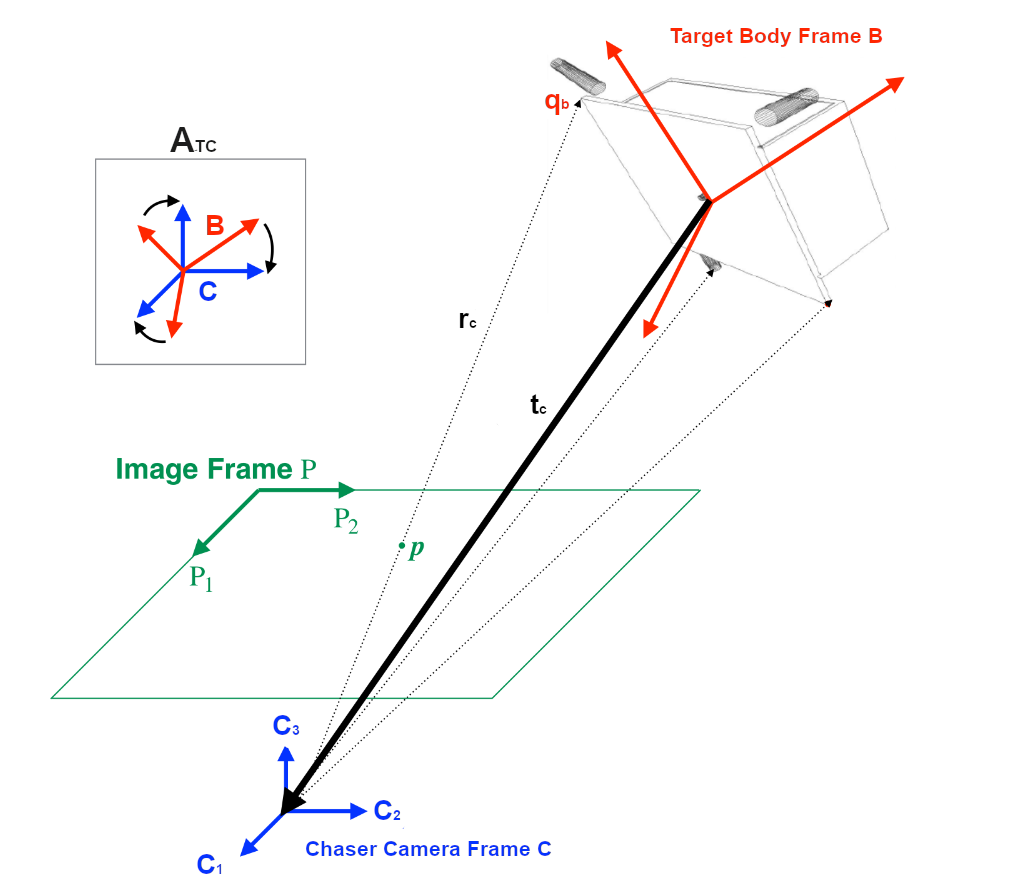
\includegraphics[width=0.72\textwidth]{gfx/poseProblem.eps}
  \caption{Schematic representation of the pose estimation problem using a monocular image \cite{Sharma2018}}
  \label{fig:theposeproblem}
\end{figure}

As discussed in \cite{D2014}, we can build several considerations on top of those two coupled equations :

\begin{itemize}
  \item the relationship between image points and pose parameter is hightly non linear and the problem of retrieving the \acrshort{3d} points from the \acrshort{2d} image can have infinite solution in under-constrained situations \cite{10.1145/358669.358692};
  \item the correspondence between $\mathbf{q_B}$ and $\mathbf{p}$ is not known \textit{a priori};
  \item the image coordinates need to be corrected for pixel's non-quadratism and lens distortion before using the perspective projection equations.
\end{itemize}

The pose estimation system thus needs the be capable of extracting the client features from the available image (image processing) to obtain measurements, namely  $\mathbf{p}$. The extracted features then needs to be matched to the correspondent elements of a client model (model matching), namely $\mathbf{q_B}$. The unknown pose then has to be estimated based on the available measurements (pose estimation).
To be able to uniquely solve equations \eqref{eq:rc} and \eqref{eq:p}, at least six correspondences between the image points and the model points are needed. \cite{10.1145/358669.358692}. The challenging part of the problem is to be able to correctly detect the most meaningful points in the \acrshort{2d} image. Usually this can be archived by employing edge detection techniques, such as the Canny edge detector \cite{10.1109/TPAMI.1986.4767851} followed by the Hough transform \cite{10.1145/361237.361242}. This approach however may be biased it applied directly to the image due to the fact that these algorithm are gradient based and are not able to correctly distinguish the foreground from the background and also requires the definition of numerous hyper-parameters which are difficult to tune for broad applicability because the imaged scene and the illumination conditions are constantly changing throughout the orbit \cite{Sharma2018}.

\subsection{General Architecture}
The architecture proposed in \cite{Sharma2018} tries to solve the pose estimation problem by:

\begin{itemize}
  \item coupling the \acrfull{wge} technique with the Sobel edge detection to perform the image processing;
  \item using feature synthesis to reduce the search space for model matching;
  \item combining a \acrshort{pnp} solver with the \acrfull{nr} method for pose estimation.
\end{itemize}

\begin{figure}[htbp]
  \centering
  \includegraphics[width=1.0\textwidth]{gfx/SVDPipeline.eps}
  \caption{The \acrshort{svd} architecture for solving the pose estimation problem \cite{Sharma2018}}
  \label{fig:svdArchitecture}
\end{figure}

As the reader can see from the schematic represented in figure \ref{fig:svdArchitecture}, the pipeline is composed from two different subsystems:
\begin{itemize}
  \item the image processing subsystem, which receive as an input a \acrshort{2d} image, distinguishing the \acrshort{sc} from the image, extract its edge features and groups them into geometric groups;
  \item the pose determination subsystems, which acceps as input the previously feature groups detected by the image processing subsystem and the \acrshort{3d} model. It then pairs the \acrshort{2d} and \acrshort{3d} geometric groups to formulate multiple correspondence hypotesis. For each hypothesis formulated, the endpoints of the line segments forming the geometric groups are used to solve equation \eqref{eq:rc} and equation \eqref{eq:p}. The five best solution then are iteratively refined by employing the \acrshort{nr} method.
\end{itemize}

Two are the most meaningful innovation the \acrshort{svd} architecture introduces:
\begin{itemize}
  \item the usage of the \acrshort{wge} technique in order to distinguish the target \acrshort{sc} from the background and for enhancing the output of the edge detection procedure bu providing a robust identification of the small as well as large edges of the \acrshort{sc};
  \item the usage of feature groups detected in the image and in the \acrshort{3d} model to solve the feature correspondence problem, which also allows the \acrshort{svd} architecture to be more computationally efficient.
\end{itemize}

\subsection{Image Processing Subsystem}
The taks of the image processing subsystem is to extract the most meaningful features from the \acrshort{2d} image a of the target \acrshort{sc}. To effectively and rapidly detect the target \acrshort{sc} edges - even in presence of the Earth in the background - an hybrid image processing subsystem is proposed in \cite{Sharma2018}.
By fusing together the \acrshort{wge} technique and classical state-of-the-art edge detection techniques the architecture proposed by Sharma \textit{et al.} is capable to provide a robust and efficient identification of the rue edges of the \acrshort{sc}.
In particular, the \acrshort{wge} technique is able to identify the a \acrfull{roi} in a more accurate and robust way with respect to state-of-art techniques. The \acrshort{roi} is detection not only makes the entire subsystem robust against the background, but also allows an automated selection of the hyper-parameters needed for the Hough transform, which will be used to detect both small and large features of the \acrshort{sc}, in contrast with state-of-the-art algorithms which rely on a single set of manually tuned hyper-parameters.
The flow of the image processing subsystem is illustrated in figure \ref{fig:imageProcessingSubsystem}.

\begin{figure}[htbp]
  \centering
  \includegraphics[width=1.0\textwidth]{gfx/imageProcessingSubsystem.eps}
  \caption{The image processing subsystem \cite{Sharma2018}}
  \label{fig:imageProcessingSubsystem}
\end{figure}

\subsubsection{\acrshort{roi} Detection}
The first thing to perform when analyzing an image is to identify a \acrshort{roi}.
The raw input image - assumed to be rectified - is firstly imported in MATLAB. After that, A Gaussian filter is applied in order to the decrease the magnitude of image noise. The Gaussian filtering can be carried out by using the MATLAB function \inlinecode{MATLAB}{imgaussfilt}. In this work, the images generated with the toolbox presented in chapter \ref{chap:second-chapter} are filtered by using a standard deviation $\sigma_X = 1.15$ before being fed to the image processing subsystem. During this work, has been observed that the choice of the $\sigma_X$ value is very important for the success of the subsequent steps, as a wrong value can highly impact the effectiveness of the \acrshort{wge} technique. Once the image has been prefiltered, is fed as input to the \acrshort{wge} block, for the computation of the target's \acrshort{roi}. The first step consist in computing the magnitude of the image gradient, $|\nabla I|$,  using the Prewitt filter for computing the image gradient (for more details about what the image gradient is, refer to appendix \ref{sec:imagegradient}).
The \acrshort{sc} can be detected in the image by observing that, under most illumination conditions, in correspondence of the target \acrshort{sc} edges the gradient variation is more pronounced with respect to the background, regardless of the fact that the background is empty or the Earth is behind.
Indeed, to detect the spacecraft, the gradient distribution is normalized using the MATLAB \inlinecode{MATLAB}{mat2gray} function, sorted into $100$ uniformly distributed bins and fitted by and exponential \acrfull{pdf}, described by the equation :

\begin{equation*}
  y = \frac{1}{\mu} e^{-\frac{x}{\mu}} \,.
\end{equation*}

By observing the result histogram, it is clearly possible to see that most of the gradient intensities are weak and corresponds to the feature in the background or on the spacecraft surface. The weak gradient pixel locations can be classified by tresholding the \acrshort{pdf} fit to the gradient histogram. The original authors suggest to use a value of $0.99$ to treshold the \acrshort{pdf}, however, for what concerns this work, all the pixel which corresponds to a cumulative distribution inferior to $0.996$ are classified as weak and set to zero instead. Once the weak gradients are set to zero, only the most prominent features of the \acrshort{sc} are present in the image, as shown in figure \ref{fig:wgeSteps}.

\begin{figure}[htbp]
  \centering
  \subfloat[Original image]{\includegraphics[width=0.45\textwidth]{gfx/FeatureDetection/chosenImage.eps}}
  \qquad
  \subfloat[Gradient detection of original image]{\includegraphics[width=0.45\textwidth]{gfx/FeatureDetection/gradientBeforeTresholding.eps}}
  \qquad
  \subfloat[Histogram of normalized gradient values]{\includegraphics[width=0.45\textwidth]{gfx/FeatureDetection/gradientDistribution.eps}}
  \qquad
  \subfloat[Output filtered image gradients]{\includegraphics[width=0.45\textwidth]{gfx/FeatureDetection/imageAfterTresholding.eps}}
  \caption{Different steps of the \acrshort{wge}}
  \label{fig:wgeSteps}
\end{figure}

By computing the \acrfull{cdf} of the vertical and horizontal gradient of the filtered image obtained by the \acrshort{wge}, we can determine the coordinates of a \acrshort{roi} where the features that yield the strongest intensity variations are located. Then, assuming that the filtered image gradient is normally distributed, the \acrshort{roi} coordinates can be found by limiting each of the previously computed \acrshort{cdf}s between $0.025$ and $0.975$ in order to enclose the central $95\%$ of the normal distribution.

\begin{figure}[htbp]
  \centering
  \includegraphics[width=0.82\textwidth]{gfx/FeatureDetection/ROI.eps}
  \caption{Result of the \acrshort{roi} detection procedure}
  \label{fig:ROI}
\end{figure}

As noted in \cite{fracchio2019}, for images having a composite background the \acrshort{roi} detection is limited by the presence of interference, so a smarter choice for selecting the bounding box limits is to treshold the \acrshort{cdf}s between $0.005$ and $0.95$. Therefore, only the central $90\%$ of the normal distribution is selected. Restricting the range however negatively affect the \acrshort{roi} detection procedure for images were the background is empty. This problem can be solved by taking into account an additional constant, equal to the $5\%$ of the mean edge length of the \acrshort{roi} for enlarging the \acrshort{roi} boundaries.

\begin{figure}[htbp]
  \centering
  \subfloat[\acrshort{roi} selected by considering only the central $90\%$ of the normal distribution]{\includegraphics[width=0.47\textwidth]{gfx/FeatureDetection/ROInoConstant.eps}}
  \qquad
  \subfloat[\acrshort{roi} enlarged by adding the $5\%$ of the mean edge length of the previously \acrshort{roi}]{\includegraphics[width=0.47\textwidth]{gfx/FeatureDetection/enlargedROI.eps}}
  \caption{Improving the \acrshort{roi} detection procedure}
  \label{fig:roicomparisons}
\end{figure}

One of the innovative features of the \acrshort{wge} technique is that, once the \acrshort{roi} is correctly determined, it is possible to compute a coarse estimation of the the relative position and line of sight even before the pose determination subsystem. By defining the diagonal length of the \acrshort{roi}, $l_{ROI}$, as:

\begin{equation}
  l_{ROI} = \sqrt{{ROI_{width}}^2 + {ROI_{height}}^2} \,,
\end{equation}

a coarse estimation of the range to the target \acrshort{sc} from the origin of the camera frame is given by :

\begin{equation}
  \norm{t_C}_2 = \frac{\nicefrac{((f_x+f_y)}{2}) L_C}{l_{ROI}} \,,
\end{equation}

were \gls{lc} denotes the diagonal characteristic length of the \acrshort{sc} \acrshort{3d} model. By knowing the coordinates of the center of the image, $[C_x, C_y]$ and the coordinates of the \acrshort{roi} center, $[B_x, B_y]$, it is possible to compute the azimuth and elevation angles ($\alpha, \beta$) from the origin of the camera frame, $C$, to the origin of the body-fixed coordinate system, $B$ :

\begin{equation}
  \alpha = \arctan{\frac{B_x - C_x}{f_x}} \,,
\end{equation}

\begin{equation}
  \beta = \arctan{\frac{B_y - C_y}{f_y}} \,.
\end{equation}

Once ($\alpha, \beta$) are known, the coarse relative position solution is given by :

\begin{equation}
  t_C
  =
  \begin{bmatrix}
    \cos(\alpha) & 0 & -\sin(\alpha) \\
    0            & 1 & 0             \\
    \sin(\alpha) & 0 & \cos(\alpha)
  \end{bmatrix}
  \begin{bmatrix}
    1 & 0            & 0           \\
    0 & \cos(\beta)  & \sin(\beta) \\
    0 & -\sin(\beta) & \cos(\beta)
  \end{bmatrix}
  \begin{bmatrix}
    0            \\
    0            \\
    \norm{t_C}_2
  \end{bmatrix} \,.
\end{equation}

\begin{figure}[htbp]
  \centering
  \includegraphics[width=0.65\textwidth]{gfx/coarsePoseEstimation.eps}
  \caption{Calculation of a coarse relative position solution using the WGE
    technique \cite{Sharma2018}}
  \label{fig:coarseRelative}
\end{figure}

\subsubsection{Feature Detection}\label{sec:featureextraction}
The aim of the feature detection is to  identify and extract from the input image a set of segments that corresponds to the true edges of the target \acrshort{sc}.
In order to extract the features from the input image, a first edge detection process is applied to the tresholded image by means of the Hough transform. When applied to the problem of detecting straight lines into an image, the Hough transform performs a shape identification through a voting procedure in the parameter space ($\rho$, $\theta$) (for more details about how the Hough transform work, the interested reader can refer to appendix \ref{sec:hough}).
When computing the Hough transform using MATLAB some parameters must be set:

\begin{itemize}
  \item the desired resolution of $\rho$ and $\theta$,
  \item the maximum number of peaks to identify in the Hough transform matrix,
  \item the expected minimum length of the the line segment, \gls{l_min},
  \item the expected minimum length of the the line segment, \gls{lambda} and the maximum gap between two points to be considered in the same line segment, \gls{lambda}.
\end{itemize}

The geometrical constraints imposed to the Hough transform are dictated by the choice of \gls{l_min} and \gls{lambda}, which are usually called hyper-parameters in the \acrshort{cv} field. Fixing a value of (\gls{l_min}, \gls{lambda}) for all the images will result into the inability of the algorithm to adapt to different distances between the camera and the target \acrshort{sc}. In fact, as the camera moves closer and closer to the target \acrshort{sc}, the latter will fill larger and larger portions of the image, and the expected lengths of its edges in the image plane are expected to grow, so a recomputation of the geometrical hyper-parameters would be needed. However, it is reasonable to hypothesize that the size of the detected \acrshort{roi} bounding box will grow too, so, in \cite{Sharma2018} is proposed to scale the geometrical hyper-parameters by using the information about the \acrshort{roi} diagonal length :

\begin{equation*}
  L_{min,Hough} = \kappa_1 l_{ROI} \ \ \ \  \lambda_{Hough} = \kappa_2 l_{ROI}  \,,
\end{equation*}

were $\kappa_1$ and $\kappa_2$ are two scalars which can be empirically estimated by performing several test simulations on ground.

The idea proposed in \cite{Sharma2018} is to tune the values of $\kappa_1$ and $\kappa_2$ in order to only extract short line segments from the tresholded image.

A second stream of features is then obtained by directly appling the Sobel operator, (for more details about what the Sobel operator is, refer to appendix \ref{sec:imagegradient}), to the unfiltered, rectified image, using the MATLAB function \inlinecode{MATLAB}{edge}. The Sobel operator is applied by imposing an intensity treshold equal to $0.04$. As proposed in \cite{fracchio2019}, in order to eliminate the pixel chunks belonging to smaller reflective elements from the output of \inlinecode{MATLAB}{edge}, it is possible to filter the output by using the MATLAB function \inlinecode{MATLAB}{bwareaopen} which, once minimum pixel number $P$ is defined, it removes all connected components (objects) that have fewer than $P$ pixels from the input binary image. In contrast with what done in \cite{fracchio2019}, which sets $P = 10$ for all images, in this work the $P$ value is computed adaptively for each image exploiting the information about the \acrshort{roi} diagonal length :

\begin{equation*}
  P = \lfloor \eta \ l_{ROI}
\end{equation*}

where $\lfloor$ is the commonly used symbol for the \inlinecode{MATLAB}{floor} operator and $\eta$ is a multiplicative constants which can be tuned empirically.
After that, the Hough transform is applied again on the output produced by the Sobel operator in order to extract line segments corresponding to the silhouette of the large components of the target \acrshort{sc}. The knowledge the \acrshort{roi} location, obtained through the \acrshort{wge} technique, is now exploited to automatically reject any line segment for which the midpoint lies outside the \acrshort{roi} itself. Also for computing the \acrfull{seh} stream of features, in \cite{Sharma2018} is advised to scale the geometrical hyper-parameters needed to compute the Hough lines by using the information about the \acrshort{roi} diagonal length :

\begin{equation*}
  L_{min,Hough} = \kappa_3 l_{ROI} \ \ \ \  \lambda_{Hough} = \kappa_4 l_{ROI}  \,,
\end{equation*}

where again, $\kappa_3$ and $\kappa_4$  are two multiplicative constants which can be fixed in an offline phase before the mission. The idea proposed in \cite{Sharma2018} is to tune the values of $\kappa_3$ and $\kappa_4$ in order to extract large line segments from the image.

\subsubsection{Merging Edges}\label{sec:mergingedges}
The output of the Hough transform often results in multiple truncated edges, especially when applied to the image processed by the \acrshort{wge}. Since fragmentation can increase uncertainty and increase the computational cost of feature matching and pose solving \cite{fracchio2019}, a section of the \acrshort{svd} architecture is dedicated to find and merge line segments which may corresponds to the same true line segment into a single line segment.
To check whether two line segments can be considered similar and merged into one single edge, it is possible to define some geometrical checks on the basis of the parameters $\rho$ and $\theta$.
Considering the two line segments represented in \ref{fig:mergeEdges}a\footnote{Note that the segments are represented in the image coordinate system, where the positive x axis points to the right, the positive y axis points downward and the positive z axis points toward the direction given by $  \mathbf{\hat{z}} = \frac{\mathbf{\hat{x}} \wedge \mathbf{\hat{y}}}{\norm{\mathbf{\hat{x}} \wedge \mathbf{\hat{y}}}}$.}, it is possible to write their polar representation in the Hough space as:

\begin{equation}
  l_1 \rho_1 = x \cos (\theta_1) +  y \sin (\theta_1) \,,
\end{equation}

\begin{equation}
  l_2 \rho_2 = x \cos (\theta_2) +  y \sin (\theta_2) \,.
\end{equation}

\begin{figure}[htbp]
  \centering
  \subfloat[Original edge]{\includegraphics[width=0.47\textwidth]{gfx/segmentsPreMerge.eps}}
  \qquad
  \subfloat[Output merged edge]{\includegraphics[width=0.47\textwidth]{gfx/segmentsAfterMerge.eps}}
  \qquad
  \caption{Merging two truncated edges \cite{Sharma2018}}
  \label{fig:mergeEdges}
\end{figure}

The conditions of similarity proposed by \cite{Sharma2018} are then:

\begin{equation}
  |\theta_1 - \theta_2| \leqslant \theta_{tresh} \,,
\end{equation}

\begin{equation}
  |\rho_1 - \rho_2| \leqslant \rho_{tresh} \,,
\end{equation}

where $\theta_{tresh}$ and $\rho_{tresh}$ are set to be equal to the resolution of $\theta$ and $\rho$ in the Hough space. In \cite{fracchio2019} is proposed to scale the value of $\rho_{tresh}$ using the information about the \acrshort{roi} diagonal length in order to improve the identification of the spacecraft true edges :

\begin{equation}
  \rho_{tresh} = \nu d_{ROI} \,,
\end{equation}

where $\nu$ is a multiplicative constant which can be set to be equal to the resolution of $\rho$ in the Hough space. In this work, this second approach has been preferred.
Furthermore, it is imposed that the Euclidean distance between the farthest pair of endpoints of the two line segments must be less than $d_{tresh}$ :

\begin{equation}
  d_{p_{1a}-p_{2b}} \leqslant d_{tresh} \,,
\end{equation}

where $d_{tresh}$ is computed for each image as half of the mean length of the detected segments :

\begin{equation}
  d_{tresh} = {\frac{1}{2}} \overline{(l_1, l_2,\ldots, l_n)} \,.
\end{equation}

If the similarity conditions are met, then the two line segments are replaced with the line $l_3$, which is the line segment which joins the two farthest endpoints of $l_1$ and $l_2$ :

\begin{equation}
  l_3 \rho_3 = x \cos (\theta_3) +  y \sin (\theta_3) \,.
\end{equation}

The Hough parameters which defines $l_3$ can be computed as follows\footnote{Note that the computation is done in the image coordinate system previously defined}. First, the angle between the positive x-axis and the joined segment is retrieved\footnote{Note that it is necessary to subtract $90^{\circ}$ from the computed angle to take into account that in the image coordinate system negative the quadrant is the upper while the positive one is the lower} :

\begin{equation}
  \alpha = 90^{\circ} - \arctan{\left(\frac{p_{1a,x}-p_{2b,x}}{p_{1a,y}-p_{2b,y}}\right)} \,,
\end{equation}

from which it follows the value of $\theta_3$

\begin{equation}
  \theta_3 = \alpha - 90^{\circ} \,.
\end{equation}

\begin{figure}[htbp]
  \centering
  \includegraphics[width=0.45\textwidth]{gfx/hough_rho_theta_diagram.eps}
  \caption{$\rho$ and $\theta$ diagram}
  \label{fig:rhotheta}
\end{figure}

Now, to find $\rho_3$ it is sufficient to compute the intersection between the line which passes trough the origin and is also perpendicular to the joined segment :

\begin{equation}
  m = \tan(\alpha)
\end{equation}

\begin{equation}
  x = \frac{m(p_{1a,x}-p_{1a,y})}{\nicefrac{1}{m} + m} \,,
\end{equation}

\begin{equation}
  y = - \frac{1}{m} x \,,
\end{equation}

\begin{equation}
  \rho_3 = x \cos (\theta_3) +  y \sin (\theta_3) \,.
\end{equation}

For what concerns the \acrshort{seh} stream instead, the \inlinecode{MATLAB}{edge} function is applied by using a treshold of $0.4$. After that, the Hough transform is applied, and a dedicated function removes all the detected lines which midpoints are located outside the \acrshort{roi}.
In figures \ref{fig:resultsMergingEdge}, \ref{fig:resultsMergingEdge2}, \ref{fig:resultsMergingEdge3} are presented some preliminary results of the edge merging procedure applied to images produced using the toolbox presented in \ref{chap:second-chapter}. The resolution of $\rho$ and $\theta$ imposed to the Hough transform are set as $0.001 d_{ROI}$ px, $5^\circ$ over the range $[-90 \ 89]$ with a maximum number of $5$ peaks over a thresold of $0.1$ for the \acrshort{wge} stream and $0.001 d_{ROI}$ px, $0.1^\circ$ over the range $[-90 \ 89]$ with a maximum number of $10$ peaks over a threshold of $0.1$ for the \acrshort{seh} stream.

\begin{figure}[htbp]
  \centering
  \subfloat[\acrshort{wge} output]{\includegraphics[width=0.47\textwidth]{gfx/FeatureDetection/wgeHough.eps}}
  \qquad
  \subfloat[\acrshort{wge} output after merging truncated edges]{\includegraphics[width=0.47\textwidth]{gfx/FeatureDetection/wgeMerged.eps}}
  \qquad
  \subfloat[\acrshort{seh} output]{\includegraphics[width=0.47\textwidth]{gfx/FeatureDetection/seHough.eps}}
  \qquad
  \caption{Results obtained applying edge detection and Hough transform on the two streams (1)}
  \label{fig:resultsMergingEdge}
\end{figure}

\begin{figure}[htbp]
  \centering
  \subfloat[\acrshort{wge} output]{\includegraphics[width=0.47\textwidth]{gfx/FeatureDetection/wgeHough3.eps}}
  \qquad
  \subfloat[\acrshort{wge} output after merging truncated edges]{\includegraphics[width=0.47\textwidth]{gfx/FeatureDetection/wgeMerged3.eps}}
  \qquad
  \subfloat[\acrshort{seh} output]{\includegraphics[width=0.47\textwidth]{gfx/FeatureDetection/seHough3.eps}}
  \qquad
  \caption{Results obtained applying edge detection and Hough transform on the two streams (2)}
  \label{fig:resultsMergingEdge2}
\end{figure}

\begin{figure}[htbp]
  \centering
  \subfloat[\acrshort{wge} output]{\includegraphics[width=0.47\textwidth]{gfx/FeatureDetection/wgeHough2.eps}}
  \qquad
  \subfloat[\acrshort{seh} output]{\includegraphics[width=0.47\textwidth]{gfx/FeatureDetection/seHough2.eps}}
  \qquad
  \caption{Case where no merging was required}
  \label{fig:resultsMergingEdge3}
\end{figure}

\subsubsection{Merge Streams}
The final step of  the feature detection procedure consist into merging the two streams of features obtained by using both the \acrshort{wge} and \acrshort{seh}. The aim of combining the two different streams is to identify different elements of the \acrshort{sc} silhouette. As stated in \cite{Sharma2018}, the uniqueness check archived in this phase resolves the issue of detecting repeated edges as encountered in previous works.
In contrast with what proposed in \cite{Sharma2018}, which suggests to detect and merge pairs of close and similar line segments separately for the two streams and merge them after, here this job is accomplished in one step. The line segments of both streams are collected together and scanned by a loop which decides what to do with the current pair being analyzed on the basis of some geometrical conditions which are set.
For example, pairs of close and similar line segments are detected and merged using conditions similar to the one imposed in section \ref{sec:mergingedges}:

\begin{equation}
  |\theta_1 - \theta_2| \leqslant \tilde{\theta}_{tresh} \,,
\end{equation}

\begin{equation}
  |\rho_1 - \rho_2| \leqslant \tilde{\rho}_{tresh} \,,
\end{equation}

where $\tilde{\rho}_{tresh}$ can be expressed as a function of the \acrshort{roi} diagonal lenght trough the multiplicative constant $\tilde{\nu}$ \cite{fracchio2019}:

\begin{equation}
  \tilde{\rho}_{tresh} = \tilde{\nu} d_{ROI} \,.
\end{equation}

Furthermore, it is imposed that the Euclidean distance between the midpoints must be less than half the length of the shorter line. With reference to figure \ref{fig:mergeEdges} :

\begin{equation}
  d_{p_{1b}-p_{2a}} \leqslant \tilde{d}_{tresh} \,,
\end{equation}

where $\tilde{d}_{tresh}$ is computed for each pair being considered as half the length of the longer line segment :

\begin{equation}
  \tilde{d}_{tresh} = {\frac{1}{2}} max(l_1, l_2) \,.
\end{equation}

If the $\tilde{d}_{tresh}$ check is failed, the loop does two more checks before passing to the next pair. The first check controls if it is being considered a case were are present two long lines which intersect. The intersection can be computed by exploiting linear algebra. Considering two lines, $l_1$ ($x_1,x_2$,$y_1$,$y_2$) and $l_2$ ($x_3,x_4$,$y_3$,$y_4$) is possible to compute the following determinants :

\begin{equation}
  dt_1 = det \left(
  \begin{bmatrix}
      1   & 1   & 1   \\
      x_1 & x_2 & x_3 \\
      y_1 & y_2 & y_3
    \end{bmatrix}
  \begin{bmatrix}
      1   & 1   & 1   \\
      x_1 & x_2 & x_4 \\
      y_1 & y_2 & y_4
    \end{bmatrix}
  \right)
\end{equation}

\begin{equation}
  dt_2 = det \left(
  \begin{bmatrix}
      1   & 1   & 1   \\
      x_1 & x_3 & x_4 \\
      y_1 & y_3 & y_4
    \end{bmatrix}
  \begin{bmatrix}
      1   & 1   & 1   \\
      x_2 & x_3 & x_4 \\
      y_2 & y_3 & y_4
    \end{bmatrix}
  \right)
\end{equation}

at this point, if $dt_1  \leqslant 0$ and $dt_2  \leqslant 0$ the two lines intersect, otherwise they do not.
If they do intersect, then only the line segment composed by joining the farthest endpoints is retained if the following condition is met:

\begin{equation}
  \epsilon = \frac{min(l_1,l_2)}{max(l_1,l_2)} > 0.25 \,.
\end{equation}

The second check instead controls if it is being considered a case were are present two long lines which are almost parallel. The parallelism is computed by exploiting the information about $\rho$ :

\begin{equation}
  \chi = 1 - \frac{min(\rho_1,\rho_2)}{max(\rho_1,\rho_2)} \,
\end{equation}

if $\chi$ is less than $0.005$ then the two lines are considered parallel and only the line segment composed by joining the farthest endpoints is retained if:

\begin{equation}
  \epsilon = \frac{min(l_1,l_2)}{max(l_1,l_2)} > 0.25 \,.
\end{equation}

Figures \ref{fig:mergeStreams1}, \ref{fig:mergeStreams2}, \ref{fig:mergeStreams3} shows the results of the merge streams procedure when applied to the images generated with the toolbox described in chapter \ref{chap:second-chapter}.

\begin{figure}[htbp]
  \centering
  \subfloat[\acrshort{wge} and Hough result]{\includegraphics[width=0.47\textwidth]{gfx/FeatureDetection/192/10.png}}
  \qquad
  \subfloat[\acrshort{seh} result]{\includegraphics[width=0.47\textwidth]{gfx/FeatureDetection/192/11.png}}
  \qquad
  \subfloat[\acrshort{wge} merged lines]{\includegraphics[width=0.47\textwidth]{gfx/FeatureDetection/192/12.png}}
  \qquad
  \subfloat[Sobel merged lines]{\includegraphics[width=0.47\textwidth]{gfx/FeatureDetection/192/13.png}}
  \qquad
  \subfloat[Merge \acrshort{wge} and Sobel]{\includegraphics[width=0.47\textwidth]{gfx/FeatureDetection/192/14.png}}
  \qquad
  \subfloat[Final result]{\includegraphics[width=0.47\textwidth]{gfx/FeatureDetection/192/15.png}}
  \qquad
  \caption{Results of the merging process (1)}
  \label{fig:mergeStreams1}
\end{figure}

\begin{figure}[htbp]
  \centering
  \subfloat[\acrshort{wge} and Hough result]{\includegraphics[width=0.47\textwidth]{gfx/FeatureDetection/214/10.png}}
  \qquad
  \subfloat[\acrshort{seh} result]{\includegraphics[width=0.47\textwidth]{gfx/FeatureDetection/214/11.png}}
  \qquad
  \subfloat[\acrshort{wge} merged lines]{\includegraphics[width=0.47\textwidth]{gfx/FeatureDetection/214/12.png}}
  \qquad
  \subfloat[Sobel merged lines]{\includegraphics[width=0.47\textwidth]{gfx/FeatureDetection/214/13.png}}
  \qquad
  \subfloat[Merge \acrshort{wge} and Sobel]{\includegraphics[width=0.47\textwidth]{gfx/FeatureDetection/214/14.png}}
  \qquad
  \subfloat[Final result]{\includegraphics[width=0.47\textwidth]{gfx/FeatureDetection/214/15.png}}
  \qquad
  \caption{Results of the merging process (2)}
  \label{fig:mergeStreams2}
\end{figure}

\begin{figure}[htbp]
  \centering
  \subfloat[\acrshort{wge} and Hough result]{\includegraphics[width=0.47\textwidth]{gfx/FeatureDetection/311/10.png}}
  \qquad
  \subfloat[\acrshort{seh} result]{\includegraphics[width=0.47\textwidth]{gfx/FeatureDetection/311/11.png}}
  \qquad
  \subfloat[\acrshort{wge} merged lines]{\includegraphics[width=0.47\textwidth]{gfx/FeatureDetection/311/12.png}}
  \qquad
  \subfloat[Sobel merged lines]{\includegraphics[width=0.47\textwidth]{gfx/FeatureDetection/311/13.png}}
  \qquad
  \subfloat[Merge \acrshort{wge} and Sobel]{\includegraphics[width=0.47\textwidth]{gfx/FeatureDetection/311/14.png}}
  \qquad
  \subfloat[Final result]{\includegraphics[width=0.47\textwidth]{gfx/FeatureDetection/311/15.png}}
  \qquad
  \caption{Results of the merging process (3)}
  \label{fig:mergeStreams3}
\end{figure}

\subsubsection{Feature Synthesis and Perceptual Grouping}
One of the innovation introduced in the \acrshort{svd} algorithm is what by the original authors has been defined as "Feature Synthesys", which allows to organize the simple segments output from the merge of the \acrshort{wge} and \acrshort{seh} streams into into high-level geometrical groups called "Perceptual Groups" in order to reduce the search space of the correspondence problem. Being able to correctly define perceptual groups is of crucial importance to have a successful pose initialization.
As stated in \cite{10.1145/358669.358692}, to uniquely solve the \acrshort{pnp} problem are required at least six correspondences between model and image points. The number of possible correspondences, so, the number of hypothetical pose solution given \textit{n} points in the image and \textit{m} points in the \acrshort{3d} model therefore can be expressed as \cite{Sharma2018}:

\begin{equation*}
  \binom{m}{6} \binom{n}{6} 6! \,.
\end{equation*}

The idea presented by Sharma \textit{et al.} so is to reduce the solutions' search space by just using a small set of high level feature groups instead of using a large number of feature point. For example, it is sufficiently safe to say that four image points may belong to a polygonal feature such as a solar panel, then a unique solution can be found by just using four correspondences. The feature synthesis implementation proposed by Sharma \textit{et al.} groups the features into five high-level perceptual groups, which, in order of increasing complexity are :

\begin{itemize}
  \item parallel pairs;
  \item proximity pairs;
  \item parallel triads;
  \item proximity triads;
  \item closed polygonal tetrads;
\end{itemize}

moreover, antennas are treated as a separate feature group.
As done for the merging procedure, the perceptual groups are recognized by examining several geometrical constraints.

\begin{figure}[htbp]
  \centering
  \subfloat[Parallel Pair]{\includegraphics[width=0.24\textwidth]{gfx/parallelPair.eps}}
  \qquad
  \subfloat[Proximity Pair]{\includegraphics[width=0.24\textwidth]{gfx/proximityPair.eps}}
  \qquad
  \subfloat[Parallel Triad]{\includegraphics[width=0.24\textwidth]{gfx/parallelTriad.eps}}
  \qquad
  \subfloat[Proximity Triad]{\includegraphics[width=0.24\textwidth]{gfx/proximityTriad.eps}}
  \qquad
  \subfloat[Closed Polygonal Tetrad]{\includegraphics[width=0.24\textwidth]{gfx/closedPolygonalTetrad.eps}}
  \qquad
  \caption{High-level feature groups \cite{Sharma2018}}
  \label{fig:highLevelGroups}
\end{figure}

Antennas are detected by selecting among all line segments only the one for which the following condition is met :

\begin{equation}
  l_1  \leqslant \tau d_{ROI} \,,
\end{equation}

where $\tau$ is a multiplicative constant, which \cite{Sharma2018} suggest to take equal to $\nicefrac{1}{3}$. Before checking if a line can be inserted into an high level feature group, is always checked if it cannot be characterized as antenna.
With reference to figure \ref{fig:highLevelGroups}a, parallelism is enforced by checking the the angular difference between the two line segments:

\begin{equation}
  \theta_{12} = |\theta_1 - \theta_2| \leqslant \theta_{max} \,,
\end{equation}

However, as suggested in \cite{fracchio2019}, to avoid detecting spurious parallel pairs it is useful to introduce two more geometric constraints, which are the minimum radial distance and the minimum lines' length ratio :

\begin{equation}
  \rho_{12} = |\rho_1 - \rho_2| \geq  \rho_{min} \,,
\end{equation}

\begin{equation}
  \epsilon_{12} = \frac{min(l_1,l_2)}{max(l_1,l_2)} \geq \epsilon_{min} \,.
\end{equation}

Proximity pairs instead are detected by checking the distance between their closest endpoints. With reference to figure  \ref{fig:highLevelGroups}b, the geometric condition checked is:

\begin{equation}
  d_{12} \leqslant d_{max} \,,
\end{equation}

where $d_{max}$ can be adaptively computed in function of the \acrshort{roi} diagonal length trough a multiplicative constant:

\begin{equation}
  d_{max} = \xi d_{ROI} \,.
\end{equation}

Furthermore, in order to prevent duplicated edges to be grouped as proximal pair, in \cite{fracchio2019} is proposed a supplementary constraint on the minimum angular difference between the two line segments being considered:

\begin{equation}
  \theta_{12} = |\theta_1 - \theta_2| \geq \theta_{min} \,.
\end{equation}

Parallel triads can be detected by selecting among all parallel pairs, the ones which shares a line segment. Similarly, proximity triads are detected by scanning all the proximity pairs and extracting the ones which shares a line segment and satisfy the following geometric condition:

\begin{equation}
  (P_{1a} - P_{3a})(P_{1b}-P_{3b}) > 0 \,.
\end{equation}

Finally, polygonal tetrads that have two segments in common are classified as closed polygonal tetrads.
Similarly, the perceptual grouping is applied to a reduced CAD model of the target \acrshort{sc}. As proposed in \cite{Sharma2018}, the CAD model introduced in chapter \ref{chap:second-chapter} is reduced to only contain a low number of features. The number of features present in the wireframe reduced modules must be tuned in order to reduce all possible pose ambiguities and to reduce the number of feature correspondence hypotheses to speed up the pose determination process. The origin of the body frame is located in correspondence of the \acrshort{cg} of the \acrshort{sc}.

\begin{figure}[htbp]
  \centering
  \subfloat[Original CAD model]{\includegraphics[width=0.45\textwidth]{gfx/cadFull.eps}}
  \qquad
  \subfloat[Reduced CAD model]{\includegraphics[width=0.45\textwidth]{gfx/wireframeModel.eps}}
  \qquad
  \caption{Full CAD model and reduced one}
  \label{fig:cadModel}
\end{figure}

Once the CAD model is input in MATLAB\footnote{The following function can be used: \url{https://www.mathworks.com/matlabcentral/fileexchange/30923-fast-stl-import-function}} and reduced, the same feature groups can be extracted from the \acrshort{3d} model by applying \acrshort{3d} geometry definitions instead of \acrshort{2d} ones. For example, parallelism can be defined using the unit vectors constructed using end-points of the lines. Similarly, proximal pairs can be defined based on the smallest possible distance between the end points of the line segments, etc.
From the \acrshort{3d} model shown in figure \ref{fig:cadModel} the following high level features have been detected :

\begin{itemize}
  \item 18 parallel pairs;
  \item 16 proximity pairs;
  \item 12 parallel triads;
  \item 11 proximity triads;
  \item 2 closed polygonal tetrads;
\end{itemize}

in addition to the five antennas and the lateral bar which have been placed on the \acrshort{sc}.

\subsection{Model Matching}
Once all feature groups are extracted from the \acrshort{3d} model and the \acrshort{2d} image, the baseline idea is to hypothesize correspondences between the endpoints of the \acrshort{3d} model and \acrshort{2d} line segments for each matching feature group pair through simple combinations. The point correspondences then are stored in a match matrix, which can be then input to the desired \acrshort{pnp} solver.The feature groups can ranked according their geometrical complexity, and only the most geometrically complex feature group detected in the image are considered.

\begin{table}[htbp]
  \centering
  \includegraphics[width=1.0\textwidth]{gfx/matchMatrix.eps}
  \caption{Expected number of rows in the match matrix (column 5) based on the most geometrically complex feature
    group detected in the image (column 1) \cite{Sharma2018}}
  \label{tab:matchMatrix}
\end{table}

In table \ref{tab:matchMatrix} is shown the number of rows the match matrix should have for a spacecraft like the tango \acrshort{sc} in a typical scenario were at lest three antennas are detected.
Unlike previous view based pose estimation techniques, in the \acrshort{svd} architecture not all possible feature matches are treated identically. Instead, a small set of matches is hypothesized and then verified, by combining most complex feature group with simplest feature groups detected in order to have enough point matches to fed to the pose solver. In particular, for \acrshort{sc}s like Tango, Sharma \textit{et al.} propose to to combine point correspondence from complex feature groups with point correspondences from the antennas feature group, since the \acrshort{sc} has several antennas which are visible from most viewing angles.

\subsection{Pose Determination}
For the pose determination step the original authors propose to couple the e\acrshort{pnp} pose solver \cite{10.1007/s11263-008-0152-6} to each combination of feature correspondence present in the match matrix to archive the five best solutions and then use those for pose refinement by using the \acrshort{nr} method to solve equations \eqref{eq:rc} and \eqref{eq:p} using each pose solution as initial guess in order to minimize the following fit error:

\begin{equation}
  \mathbf{E_i} = \left[u_i - \left( \frac{x_C}{z_C} f_x + C_x \right) , \left( v_i - \frac{y_C}{z_C} f_y + C_y \right) \right]  \mbox{ for } i=1,...,n \,.
  \label{eq:errorFIT}
\end{equation}

In this work however it has been opted to use a built-in MATLAB function which returns orientation and position of a calibrate camera by means of a P3P solver \cite{XiaoShanGao2003} coupled with a RANSAC algorithm for outlier rejection \cite{Torr2000} in a coordinate system which is the one of the map input to the function (so to speak, the wireframe \acrshort{3d} model previously introduced). The P3P solver produces up to four symmetrical solutions using three points. Less solution can be produced if some geometrical and algebraic conditions are met.
Since the \acrshort{pnp} is prone to error if any outliers are present in the set of give point correspondences, the RANSAC is used to make the final solution more robust.

\section{Conclusions}
This chapter is concluded showing to the reader some cases of successful pose initialization when using the \acrshort{svd} architecture which has been described and analyzed trough the whole chapter. In the table \ref{tab:svdParameters} the interested reader can see the values of some of the \acrshort{roi} parameters which have been described in the trough the previous sections used to tune the \acrshort{svd} algorithm in order to analyze the image produced with the toolbox presented in chapter \ref{chap:second-chapter}.

\begin{table}[htbp]
  \centering
  \begin{tabular}{cc}
    \hline
    \hline
    Symbol                   & Value          \\
    \hline
    $\kappa_1$               & $0.031$        \\
    \hline
    $\kappa_2$               & $0.0085$       \\
    \hline
    $\kappa_3$               & $0.086$        \\
    \hline
    $\kappa_4$               & $0.0146$       \\
    \hline
    $\eta$                   & $0.03$         \\
    \hline
    $\theta_{tresh}$         & \ang{10}       \\
    \hline
    $\nu$                    & $0.1$          \\
    \hline
    $\tilde{\theta}_{tresh}$ & \ang{10}       \\
    \hline
    $\tilde{\nu}$            & $0.129$        \\
    \hline
    $\theta_{max}$           & \ang{10}       \\
    \hline
    $\rho_{min}$             & $0.05 d_{ROI}$ \\
    \hline
    $\epsilon_{min}$         & 0.7            \\
    \hline
    $\xi$                    & $0.03$         \\
    \hline
    $\theta_{min}$           & \ang{10}       \\
    \hline
    \hline
  \end{tabular}
  \caption{Parameters used to tune the \acrshort{svd} algorithm}
  \label{tab:svdParameters}
\end{table}

The accuracy of the estimated pose can be evaluated by defining the following errors:

\begin{equation}
  \mathbf{E_t} = |\mathbf{t_c}^{true} - \mathbf{t_c}^{est}|
\end{equation}

\begin{equation}
  \mathbf{A_{diff}} = \mathbf{A_{TC}}^{est}(\mathbf{A_{TC}}^{true})^T
\end{equation}

where $\mathbf{E_t}$ represents the absolute difference between the ground truth position of the \acrshort{sc} (the one imposed at the moment when the image was generated) and the estimated position provided by the pose solution, and $\mathbf{A_{diff}}$ is the \acrshort{dcm} representing the relative rotation between the ground truth value (the one imposed at the moment when the image was generated) and the estimated value of $\mathbf{A_{TC}}$.

\begin{figure}[htpb]
  \setbox1=\hbox{\includegraphics[width=0.45\textwidth]{gfx/PoseDetermination/trial49modelMap.eps}}% The smaller image
  \setbox2=\hbox{\includegraphics[width=0.45\textwidth]{gfx/PoseDetermination/cameraWRTSC49.eps}}% The larger image
  {\,} \hfill
  \subfloat[Map superposed to the image]{%
    \raisebox{0.5\ht2-0.5\ht1}{\includegraphics[width=0.45\textwidth]{gfx/PoseDetermination/trial49modelMap.eps}}} \hfill
  \subfloat[\acrshort{3d} camera pose in map coordinates]{%
    \includegraphics[width=0.45\textwidth]{gfx/PoseDetermination/cameraWRTSC49.eps}} \hfill
  {\,}
  \caption{Case of successful pose initialization (1)}
  \label{fig:EVVAI1}
\end{figure}

\begin{figure}[htpb]
  \setbox1=\hbox{\includegraphics[width=0.45\textwidth]{gfx/PoseDetermination/trial214modelMap.eps}}% The smaller image
  \setbox2=\hbox{\includegraphics[width=0.45\textwidth]{gfx/PoseDetermination/cameraWRTSC214.eps}}% The larger image
  {\,} \hfill
  \subfloat[Map superposed to the image]{%
    \raisebox{0.5\ht2-0.5\ht1}{\includegraphics[width=0.45\textwidth]{gfx/PoseDetermination/trial214modelMap.eps}}} \hfill
  \subfloat[\acrshort{3d} camera pose in map coordinates]{%
    \includegraphics[width=0.45\textwidth]{gfx/PoseDetermination/cameraWRTSC214.eps}} \hfill
  {\,}
  \caption{Case of successful pose initialization (2)}
  \label{fig:EVVAI2}
\end{figure}

\begin{figure}[htpb]
  \setbox1=\hbox{\includegraphics[width=0.45\textwidth]{gfx/PoseDetermination/trial212modelMap.eps}}% The smaller image
  \setbox2=\hbox{\includegraphics[width=0.45\textwidth]{gfx/PoseDetermination/cameraWRTSC212.eps}}% The larger image
  {\,} \hfill
  \subfloat[Map superposed to the image]{%
    \raisebox{0.5\ht2-0.5\ht1}{\includegraphics[width=0.45\textwidth]{gfx/PoseDetermination/trial212modelMap.eps}}} \hfill
  \subfloat[\acrshort{3d} camera pose in map coordinates]{%
    \includegraphics[width=0.45\textwidth]{gfx/PoseDetermination/cameraWRTSC212.eps}} \hfill
  {\,}
  \caption{Case of successful pose initialization (3)}
  \label{fig:EVVAI3}
\end{figure}

\begin{figure}[htpb]
  \setbox1=\hbox{\includegraphics[width=0.45\textwidth]{gfx/PoseDetermination/trial311modelMap.eps}}% The smaller image
  \setbox2=\hbox{\includegraphics[width=0.45\textwidth]{gfx/PoseDetermination/cameraWRTSC311.eps}}% The larger image
  {\,} \hfill
  \subfloat[Map superposed to the image]{%
    \raisebox{0.5\ht2-0.5\ht1}{\includegraphics[width=0.45\textwidth]{gfx/PoseDetermination/trial311modelMap.eps}}} \hfill
  \subfloat[\acrshort{3d} camera pose in map coordinates]{%
    \includegraphics[width=0.45\textwidth]{gfx/PoseDetermination/cameraWRTSC311.eps}} \hfill
  {\,}
  \caption{Case of successful pose initialization (4)}
  \label{fig:EVVAI4}
\end{figure}
\cleardoublepage{}
\chapter{Results\label{chap:fourth-chapter}}
\begin{quotation}
  {\footnotesize
    \noindent{\emph{``Most good programmers do programming not because they expect to get paid or get adulation by the public, but because it is fun to program.''\\}
    }
    \begin{flushright}
      Linus Torvalds
    \end{flushright}
  }
\end{quotation}
\vspace{0.5cm}

In this chapter the reader is first be presented with a qualitative analysis of the images produced with the toolbox illustrated in Chapter~\ref{chap:second-chapter}. After that, the preliminary validation of the \acrshort{svd} algorithm when applied to the same images is discussed.

\section{Qualitative Assessment}
The aim of the toolbox presented in Chapter~\ref{chap:second-chapter} was to create batches of realistic images of a given CAD of a \acrshort{sc} in order to cope with the lack of an actual facility to produce images from a scale \acrshort{3d} printed model of the target itself, as done in \cite{Beierle2019}. Validating the goodness of the generated images is extremely difficult because of the actual lack of high-resolution and high-quality images taken in orbit by a real camera of a real \acrshort{sc}. So, the more realistic intent of this evaluation is therefore to compare the generated images to the images found in the SPEED data-set \footnote{The SPEED data-set is freely available at \url{https://kelvins.esa.int/satellite-pose-estimation-challenge/}.}, in order to identify similarities and differences. As proposed in \cite{pangufinal}, the images can be compared in three ways:

\begin{itemize}
  \item visual comparison;
  \item image histogram comparison;
  \item basic feature extraction using a Sobel edge detector.
\end{itemize}

Unfortunately, the orbit and the true pose but more importantly the illumination conditions of each of the images contained in the SPEED data-set was not available at the time of writing this thesis, so it is impossible to present to the reader a one-to-one comparison. Still, it is worth to compare images which can be reasonably considered similar.

\begin{figure}[htbp]
  \centering
  \subfloat[Unfiltered image.]{\includegraphics[width=0.45\textwidth]{gfx/comparison/comp1/1.eps}}
  \qquad
  \subfloat[Unfiltered image.]{\includegraphics[width=0.45\textwidth]{gfx/comparison/comp1/2.eps}}
  \qquad
  \subfloat[Histogram.]{\includegraphics[width=0.45\textwidth]{gfx/comparison/comp1/3.eps}}
  \qquad
  \subfloat[Histogram.]{\includegraphics[width=0.45\textwidth]{gfx/comparison/comp1/4.eps}}
  \qquad
  \subfloat[Sobel image.]{\includegraphics[width=0.45\textwidth]{gfx/comparison/comp1/5.eps}}
  \qquad
  \subfloat[Sobel image.]{\includegraphics[width=0.45\textwidth]{gfx/comparison/comp1/6.eps}}
  \qquad
  \caption{Comparison between the SPEED data-set (left) and images generated using the toolbox presented in Chapter~\ref{chap:second-chapter} (right), (1).}
  \label{fig:comparison1}
\end{figure}

\begin{figure}[htbp]
  \centering
  \subfloat[Unfiltered image.]{\includegraphics[width=0.45\textwidth]{gfx/comparison/comp2/1.eps}}
  \qquad
  \subfloat[Unfiltered image.]{\includegraphics[width=0.45\textwidth]{gfx/comparison/comp2/2.eps}}
  \qquad
  \subfloat[Histogram.]{\includegraphics[width=0.45\textwidth]{gfx/comparison/comp2/3.eps}}
  \qquad
  \subfloat[Histogram.]{\includegraphics[width=0.45\textwidth]{gfx/comparison/comp2/4.eps}}
  \qquad
  \subfloat[Sobel image.]{\includegraphics[width=0.45\textwidth]{gfx/comparison/comp2/5.eps}}
  \qquad
  \subfloat[Sobel image.]{\includegraphics[width=0.45\textwidth]{gfx/comparison/comp2/6.eps}}
  \qquad
  \caption{Comparison between the SPEED data-set (left) and images generated using the toolbox presented in Chapter~\ref{chap:second-chapter} (right), (2).}
  \label{fig:comparison2}
\end{figure}

\begin{figure}[htbp]
  \centering
  \subfloat[Unfiltered image.]{\includegraphics[width=0.45\textwidth]{gfx/comparison/comp3/1.eps}}
  \qquad
  \subfloat[Unfiltered image.]{\includegraphics[width=0.45\textwidth]{gfx/comparison/comp3/2.eps}}
  \qquad
  \subfloat[Histogram.]{\includegraphics[width=0.45\textwidth]{gfx/comparison/comp3/3.eps}}
  \qquad
  \subfloat[Histogram.]{\includegraphics[width=0.45\textwidth]{gfx/comparison/comp3/4.eps}}
  \qquad
  \subfloat[Sobel image.]{\includegraphics[width=0.45\textwidth]{gfx/comparison/comp3/5.eps}}
  \qquad
  \subfloat[Sobel image.]{\includegraphics[width=0.45\textwidth]{gfx/comparison/comp3/6.eps}}
  \qquad
  \caption{Comparison between the SPEED data-set (left) and images generated using the toolbox presented in Chapter~\ref{chap:second-chapter} (right), (3).}
  \label{fig:comparison3}
\end{figure}

\begin{figure}[htbp]
  \centering
  \subfloat[Unfiltered image.]{\includegraphics[width=0.45\textwidth]{gfx/comparison/comp4/1.eps}}
  \qquad
  \subfloat[Unfiltered image.]{\includegraphics[width=0.45\textwidth]{gfx/comparison/comp4/2.eps}}
  \qquad
  \subfloat[Histogram.]{\includegraphics[width=0.45\textwidth]{gfx/comparison/comp4/3.eps}}
  \qquad
  \subfloat[Histogram.]{\includegraphics[width=0.45\textwidth]{gfx/comparison/comp4/4.eps}}
  \qquad
  \subfloat[Sobel image.]{\includegraphics[width=0.45\textwidth]{gfx/comparison/comp4/5.eps}}
  \qquad
  \subfloat[Sobel image.]{\includegraphics[width=0.45\textwidth]{gfx/comparison/comp4/6.eps}}
  \qquad
  \caption{Comparison between the SPEED data-set (left) and images generated using the toolbox presented in Chapter~\ref{chap:second-chapter} (right), (4).}
  \label{fig:comparison4}
\end{figure}

In Figures~\ref{fig:comparison1}, \ref{fig:comparison2}, \ref{fig:comparison3} are presented three simulated images of the Tango \acrshort{sc} on a black background.
Overall, it is possible to recognize that the images belonging to the SPEED shows a better representation of the external look of the \acrshort{sc}, for both the solar panels, the external appendages and the external structures. This is not an issue of the technique used to render the images by itself, but merely depends from the availability of adequate textures to render the \acrshort{sc}. Usually, the manufacturer makes available textures of the external look of the whole \acrshort{sc}. For this project unfortunately, due to the unavailability of said textures, the whole look of had to be recreated by hand, doing several experiments and comparisons. This is particularly visible when looking at solar panels, where the SPEED images are of an order of magnitude superior in terms of accuracy and realness of what is being represented.
Despite said issues however, by looking at the forms of the histograms it is possible to recognize that histograms belonging to the SPEED images and histograms belonging to the images used though this project are essentially similar. They both shows the same exponential behavior. The images belonging to the SPEED data-set shows an overall greater concentration of dark values with respect to the ones generated with the toolbox presented in Chapter~\ref{chap:second-chapter}. This is likely to be due to slightly different scenes being represented in terms of illumination conditions and shadows.
The Sobel edge images are also very similar. The images generated for this project presents a slightly higher level of noise (recognizable by the more presence of little white pixels). This can be due to different $\sigma^2$ value used to add Gaussian white noise to the image during the post-processing phase. As said for the textures, this is not an issue of the technique employed to render the image. Usually the amount of noise to add to the image during the post-processing phase depends on the intrinsic characteristics of the camera which is being simulated. For this work has been decided to mimic as much as possible the behavior of the SPEED data-set, but in general, the amount of noise to add is a parameter which can be tuned to obtain the desired result.
Lastly, in Figure~\ref{fig:comparison4} is showed a comparison were the Earth is in the background. As it can be clearly seen by the reader, the Earth is represented more accurately in the SPEED data-set, but this is simply due to the fact that for the SPEED data-set the Earth images comes from actually real space imagery. As described in \cite{Sharma2019}, the Earth images used for the SPEED data-set are composed by 72 actual images of the Earth captured by the Himawari-8 geostationary meteorological satellite. The 72 images each provide a \num{100e6} pixels resolution disk-view of the Earth and were taken 10 minutes apart from each other over a period of 12 hours. The quality the Earth has in the images generated with the toolbox developed during this work can be enhanced by using a texture with an higher resolution, however this comes at the cost of long rendering times and greater RAM usage for rendering the single image. Generating one single image where the Earth is present in the background takes approximately \SI{3}{\s} and occupy \textit{circa} $2$ Gb of RAM on an Intel Core i7-4500U CPU when using mercator images rescaled to $21600 \times 10800$ pixel resolution. Better results can be achieved using the full $43200 \times 21600$ pixel original mercator images but rendering times as well as RAM usage would grow too much for the generation of a data-set of hundreds of images on the previously mentioned H/W. Obviously, this limit can be overcome by employing a more suitable workstation.

\section{\acrshort{svd} Architecture Tests}
A further validation of the generated data-set can be obtained by analyzing the synthetic images using a \acrshort{cv} algorithm. In fact, if the quality of the generated images is poor, where for poor it is intended not being photorealistic, the \acrshort{cv} algorithm will not work consistently. Among all state-of-the-art \acrshort{cv} algorithms available, the \acrshort{svd} algorithm has been selected because of its simplicity and effectiveness. The identification of a correct \acrshort{roi} is of vital importance since the edge detection process as well as the merging edges block depends on geometrical parameters which are set as multiplicative constants of the diagonal length of the \acrshort{roi}. From a first batch of tests realized using the images generated with the toolbox presented in Chapter~\ref{chap:second-chapter}, the \acrshort{roi} detection performances of the \acrshort{wge} technique are consistent with what found in \cite{Sharma2018} and \cite{fracchio2019}. When the image has a black or nearly black background, the results of the \acrshort{wge} are very good, and in almost all cases it's capable of identifying the correct \acrshort{roi}. However, the presence of a composite background, such as it is Earth, in some cases negatively affects the performances of the \acrshort{wge} technique. This is due to the fact that the presence of the Earth produces spurious element in the gradient image, which are not eliminated by the filtering procedure. This particular behavior can be observed for example in Figures~\ref{fig:roiResults1}a, \ref{fig:roiResults1}h and \ref{fig:roiResults2}e.

\begin{figure}[htpb]
  \centering
  \subfloat[]{\includegraphics[width=0.47\textwidth]{gfx/results/prisma/101/9.png}}
  \qquad
  \subfloat[]{\includegraphics[width=0.47\textwidth]{gfx/results/prisma/111/9.png}}
  \qquad
  \subfloat[]{\includegraphics[width=0.47\textwidth]{gfx/results/prisma/112/9.png}}
  \qquad
  \subfloat[]{\includegraphics[width=0.47\textwidth]{gfx/results/prisma/113/9.png}}
  \qquad
  \subfloat[]{\includegraphics[width=0.47\textwidth]{gfx/results/prisma/114/9.png}}
  \qquad
  \subfloat[]{\includegraphics[width=0.47\textwidth]{gfx/results/prisma/115/9.png}}
  \qquad
  \subfloat[]{\includegraphics[width=0.47\textwidth]{gfx/results/prisma/116/9.png}}
  \qquad
  \subfloat[]{\includegraphics[width=0.47\textwidth]{gfx/results/prisma/117/9.png}}
  \qquad
  \caption{ROI detection tests.}
  \label{fig:roiResults1}
\end{figure}

\begin{figure}[htpb]
  \centering
  \subfloat[]{\includegraphics[width=0.47\textwidth]{gfx/results/prisma/104/9.png}}
  \qquad
  \subfloat[]{\includegraphics[width=0.47\textwidth]{gfx/results/prisma/161/9.png}}
  \qquad
  \subfloat[]{\includegraphics[width=0.47\textwidth]{gfx/results/prisma/162/9.png}}
  \qquad
  \subfloat[]{\includegraphics[width=0.47\textwidth]{gfx/results/prisma/163/9.png}}
  \qquad
  \subfloat[]{\includegraphics[width=0.47\textwidth]{gfx/results/prisma/164/9.png}}
  \qquad
  \subfloat[]{\includegraphics[width=0.47\textwidth]{gfx/results/prisma/165/9.png}}
  \qquad
  \subfloat[]{\includegraphics[width=0.47\textwidth]{gfx/results/prisma/166/9.png}}
  \qquad
  \subfloat[]{\includegraphics[width=0.47\textwidth]{gfx/results/prisma/169/9.png}}
  \qquad
  \caption{ROI detection tests.}
  \label{fig:roiResults2}
\end{figure}

\begin{figure}[htpb]
  \centering
  \includegraphics[width=1.0\textwidth]{gfx/results/prisma/101/8Select.png}
  \caption{Gradient image of Figure~\ref{fig:roiResults1}a. Left is normalized gradient, right is normalized gradient after tresholding. The spurious points not filtered by the \acrshort{wge} technique are enclosed in the red box.}
\end{figure}

\begin{figure}[htpb]
  \centering
  \includegraphics[width=1.0\textwidth]{gfx/results/prisma/117/8Select.png}
  \caption{Gradient image of Figure~\ref{fig:roiResults1}h. Left is normalized gradient, right is normalized gradient after tresholding. The spurious points not filtered by the \acrshort{wge} technique are enclosed in the red box.}
\end{figure}

\begin{figure}[htpb]
  \centering
  \includegraphics[width=1.0\textwidth]{gfx/results/prisma/164/8Select.png}
  \caption{Gradient image of Figure~\ref{fig:roiResults2}e. Left is normalized gradient, right is normalized gradient after tresholding. The spurious points not filtered by the \acrshort{wge} technique are enclosed in the red box.}
\end{figure}

A failure in the detection of a \acrshort{roi} involves the impossibility of rejecting spurious lines which do not belong to the silhouette of the \acrshort{sc} (as can be observed in Figures~\ref{fig:edgeDetection101}, \ref{fig:edgeDetection117} and \ref{fig:edgeDetection164}), and which would have been rejected in the case of a correct \acrshort{roi} selection. Moreover, it also affects the performances of the whole architecture, since all the quantities which are computed as multiplicative constants of the \acrshort{roi} diagonal length will be biased. On one hand, one could think to increase more the filtering depth of the image, but on the other hand this will penalize too much the analysis of images which do not have a composite background.

\begin{figure}[htpb]
  \centering
  \includegraphics[width=0.82\textwidth]{gfx/results/prisma/101/15.png}
  \caption{Edge detection on Figure~\ref{fig:roiResults1}a.}
  \label{fig:edgeDetection101}
\end{figure}

\begin{figure}[htpb]
  \centering
  \includegraphics[width=0.82\textwidth]{gfx/results/prisma/117/15.png}
  \caption{Edge detection on Figure~\ref{fig:roiResults1}h.}
  \label{fig:edgeDetection117}
\end{figure}

\begin{figure}[htpb]
  \centering
  \includegraphics[width=0.82\textwidth]{gfx/results/prisma/164/15.png}
  \caption{Edge detection on Figure~\ref{fig:roiResults2}e.}
  \label{fig:edgeDetection164}
\end{figure}

For what concerns the edge detection procedure instead, as observed in \cite{Sharma2018}, further improvements must be made because it is still susceptible to producing spurious edges in some corner cases. Despite this being bad from the point of view of the \acrshort{cv} algorithm, this is good for what concerns the verification of the generated data-set, which shows the same kind of issues the SPEED data-set has. In particular, it has been observed during this work that the most critical images are the ones where the solar panels are clearly visible or when the target \acrshort{sc} is far from the camera. Regarding the former case, it is particularly evident from Figure~\ref{fig:edgeDetection204}b that the culprit is likely due to the Sobel edge detector. While all the spurious points belonging to the solar panels are filtered during by the \acrshort{wge} stream, they are not in the Sobel stream. As a result, when applying the Hough transform some spurious edges are detected which are not rejected since they fall inside the \acrshort{roi}. During the work on this thesis, some efforts have been made to cope with this issue which however has not been completely resolved, from what can bee seen in Figure~\ref{fig:edgeDetection204}c. On one hand, more tresholds could be introduced into the image processing subsystem to take into account the presence of short spurious line and and remove them. On the other hand however, is really hard to fine tune those tresholds in order to not remove other short edges which instead are useful, such as antennas.

\begin{figure}[htpb]
  \centering
  \subfloat[\acrshort{wge} stream output.]{\includegraphics[width=0.47\textwidth]{gfx/results/prisma/204/10.png}}
  \qquad
  \subfloat[\acrshort{seh} stream output.]{\includegraphics[width=0.47\textwidth]{gfx/results/prisma/204/11.png}}
  \qquad
  \subfloat[\acrshort{wge} and \acrshort{seh} streams after the merge stream procedure.]{\includegraphics[width=0.47\textwidth]{gfx/results/prisma/204/15.png}}
  \qquad
  \caption{Image where the image processing subsystem contained spurious edges due to the presence of the solar panels.}
  \label{fig:edgeDetection204}
\end{figure}

There are also some particular attitudes where the Hough transform fails on the \acrshort{wge} filtered image, if the inter-spacecraft distance is relatively far. Taking as an example what's shown in Figure~\ref{fig:edgeDetection82} this can be likely due to the fact that the initial blur done to in order to filter out noise makes edges of the \acrshort{sc} harder to distinguish for the Hough transform. So, in general, the algorithm will loose accuracy as the relative distance grows.

\begin{figure}[htpb]
  \centering
  \subfloat[Normalized gradient after tresholding.]{\includegraphics[width=0.47\textwidth]{gfx/results/prisma/82/8aftertresholding.png}}
  \qquad
  \subfloat[\acrshort{wge} and Hough result.]{\includegraphics[width=0.47\textwidth]{gfx/results/prisma/82/10.png}}
  \qquad
  \subfloat[\acrshort{seh} result.]{\includegraphics[width=0.47\textwidth]{gfx/results/prisma/82/11.png}}
  \qquad
  \subfloat[Final result.]{\includegraphics[width=0.47\textwidth]{gfx/results/prisma/82/15.png}}
  \qquad
  \caption{Image where the image processing subsystem contained not correctly detected edges.}
  \label{fig:edgeDetection82}
\end{figure}

In Figures~\ref{fig:translationalErrorHist} and \ref{fig:rotationalErrorHist} are showed the histograms of the translational an the rotational errors computed over a set of 50 images. The mean values obtained are \SI{0.2506}{\m} for the translational error and $0.0528^\circ$ for the rotational error respectively.

\begin{figure}[htpb]
  \centering
  \includegraphics[width=0.9\textwidth]{gfx/plotError/transHist.eps}
  \caption{Translational Error (histogram).}
  \label{fig:translationalErrorHist}
\end{figure}

\begin{figure}[htpb]
  \centering
  \includegraphics[width=0.9\textwidth]{gfx/plotError/rotHist.eps}
  \caption{Rotational Error (histogram).}
  \label{fig:rotationalErrorHist}
\end{figure}

Figures~\ref{fig:transAndDist} and \ref{fig:rotAndDist} instead shows the variation of the translational and rotational error as the inter-spacecraft distance increases. While for the translational error there is an increasing trend as the relative distance grows, there isn't any evince of a trend for what concerns the rotational error.

\begin{figure}[htpb]
  \centering
  \includegraphics[width=0.9\textwidth]{gfx/plotError/transAndDist.eps}
  \caption{Translational error related to inter-spacecraft distance.}
  \label{fig:transAndDist}
\end{figure}

\begin{figure}[htpb]
  \centering
  \includegraphics[width=0.9\textwidth]{gfx/plotError/rotAndDist.eps}
  \caption{Rotational error related to inter-spacecraft distance.}
  \label{fig:rotAndDist}
\end{figure}

Lastly, Figure~\ref{fig:c3c2c1} shows the variation of the error with respect to camera axis. As it can be seen, there is no evidence of a privileged axis which behaves better or worse with respect to the others.

\begin{figure}[htpb]
  \centering
  \includegraphics[width=0.9\textwidth]{gfx/plotError/c3c2c1.eps}
  \caption{Error with respect to camera axis.}
  \label{fig:c3c2c1}
\end{figure}

\cleardoublepage{}

%%%%%%%%%%%%%%%%%%%%%%%%%%%%%% Conclusion
\chapter*{Conclusions}
\addcontentsline{toc}{chapter}{Conclusions}
\markboth{Conclusions}{Conclusions}
%Si mostrano le prospettive future di ricerca nell’area dove si è svolto il lavoro. 
%Nelle conclusioni si deve richiamare l’area, lo scopo della tesi, cosa è stato fatto, come si valuta quello che si è fatto e si enfatizzano le prospettive future e per mostrare come andare avanti nell’area di studio.

\cleardoublepage{}

%%%%%%%%%%%%%%%%%%%%%%%%%%%%%% Bibliography
\bibliographystyle{plain}
\bibliography{bibliography}
\cleardoublepage{}

%%%%%%%%%%%%%%%%%%%%%%%%%%%%%% Appendices
\appendix
%%% Appendix A
\chapter{First appendix: Attitude and Orbit Simulator \label{app:first-appendix}}


\cleardoublepage{}
%%% Appendix B
\chapter{Second appendix: Random Rotation Matrix Generation \label{app:second-appendix}}
\section{Kinematics}
In this section the kinematics representation used for the simulation will briefly be descripted. Two approach has been taken : 
\begin{itemize}
 \item [-] The DCM representation
 \item [-] The quaternion representation
\end{itemize}

\subsection{Direct Cosine Matrix}
The direct cosine matrix, or attitude matrix, gives the transformation of a vector from a reference frame $N$ to another reference frame $O$ : 

\begin{equation}
 \mathbf{r_{O}} = \mathbf{A_{ON}} \mathbf{r_{N}}
\end{equation}

So, if we consider the spacecraft body frame and the inertial frame, then we can write the relation between the two frames as : 

\begin{equation}
 \mathbf{r_{B}} = \mathbf{A_{B/N}} \mathbf{r_{N}}
\end{equation}

As it is demonstrated in Ref. \cite{Markley2014}, we can express the time dependence of the attitude matrix by writing the rotation from the body frame to the inertial frame as : 

\begin{equation}
 \dot{A}_{B/N}= - [\omega_{B/N} \times]A_{B/N} 
\end{equation}

where $[\omega_{B/N} \times]$ is the skew-symmetric cross product matrix containing the components of the angular velocity vector : 

\begin{equation*}
 \mathbf{[\omega \times]} =
                                \begin{bmatrix}
                                    0 & -\omega_{B/N_{3}} & \omega_{B/N_{2}} \\
                                    \omega_{B/N_{3}} & 0 & -\omega_{B/N_{1}} \\
                                    -\omega_{B/N_{2}} & \omega_{B/N_{1}} & 0
                                \end{bmatrix}
\end{equation*}

Thus, by integrating this relation, we can get full attitude at every iteration.

\subsection{Quaternions}
Quaternions are another way to parametrize the attitude of a rigid body in space. They are commonly used for control purpose due to the fact that they don't have kinematics singularities.
A quaternion is a four-component vector with some additional operations defined on it. A quaternion $\mathbf{q}$ has a three-vector part $\mathbf{q_{1:3}}$ and a scalar part $q_{4}$ : 

\begin{equation*}
 \mathbf{q} =
                                \begin{bmatrix}
                                    q_{1}\\
                                    q_{2}\\
                                    q_{3}\\
                                    q_{4}\\
                                \end{bmatrix}
\end{equation*}

The kinematic equation for the quaternion can be written as :

\begin{equation}
 \label{eq:quaternion}
 \dot{q} = \frac{1}{2} \mathbf{\varXi(\mathbf{q})} \mathbf{\omega_{B/N}}
\end{equation}

where $\mathbf{\varXi(\mathbf{q})}$ is defined as 

\begin{equation*}
 \mathbf{\varXi(\mathbf{q})} =
                                \begin{bmatrix}
                                   q_4 & -q_3 & q_2\\
                                   q_3 & q_4 & -q_1\\
                                  -q_2 & q_1 & q_4\\
                                  -q_1 & -q_2 & -q_3\\
                                \end{bmatrix}
\end{equation*}

By integrating Eq. \ref{eq:quaternion} can get the full attitude at every iteration in terms of quaternion.

\section{Dynamics}
\subsection{Euler Equations}
The dynamics of a rigid body which is tumbling into space can be modeled by mean of the well known Euler equations : 

\begin{equation}
  \mathbf{\omega_B} = \mathbf{(I_B)}^{-1} [\mathbf{L_B} - \mathbf{\omega_b}  \wedge (\mathbf{I_B} \mathbf{\omega_b})
\end{equation}

where \textbf{$\omega_B$} is the angular velocity vector of the spacecraft in body frame, \textbf{$I_B$} is the inertia tensor of the spacecraft in body frame and \textbf{$L_B$} are the external torques acting on the spacecraft due to  external disturbances and control torques.

\subsection{Environmental Disturbances} \label{sec:disturbances}
The external disturbances acting on spacecraft placed in a LEO orbit are basically four and are due to :

\begin{itemize}
  \item[-] Gravity Gradient
  \item[-] Magnetic Field 
  \item[-] Solar Radiation Pressure
  \item[-] Aerodynamic Drag
\end{itemize}

Details about how those torques have been mathematically modeled will be given in the following sections.

\subsubsection{Gravity Gradient}
Any non-symmetrical rigid body in a gravity field is subject to a gravity-gradient torque.
If we consider a rigid spacecraft, the torque due to the gravity gradient about the spacecraft's center of mass can be modeled as :

\begin{equation}
 \mathbf{L_{gg}} = \frac{3 \ mu}{r^3} \mathbf{n} \wedge (\mathbf{I} \ \mathbf{n})
\end{equation}

where $\mu$ is the Eart's gravitational constant, $\textbf{r}$ is the radius vector from the center of the Earth, thus $r \equiv \Vert{\textbf{r}}\Vert$, $\textbf{I}$ is the inertia tensor in body frame and $\textbf{n}$ is the body frame representation of a nadir-pointing unit vector.\\
Further details about the model can be found in reference \cite{Markley2014}.

\subsubsection{Earth's Magnetic Field}
The torque generated by a magnetic dipole $\textbf{m}$ in a magnetic field $\textbf{B}$ is

\begin{equation}
 \mathbf{L_{mag}} = \mathbf{m} \wedge \mathbf{B}
 \label{eq:magfield}
\end{equation}

where $\mathbf{B}$ is the magnetic field in the body frame.
The most basic source of a magnetic dipole is a current loop. A current of I amperes flowing in a planar loop of area A produces a dipole moment of magnitude m=IA in the direction normal to the plane of the loop and satisfying a right-hand rule.
When $\textbf{m}$ is in $Am^2$ and the magnetic field is specified in Tesla, Eq. \ref{eq:magfield} gives the torque in $Nm$. If there are N turns of wire in the loop, the dipole moment has magnitude m=NIA (such as the case of a magnetic torquer).
To model $\textbf{B}$ either the full IGRF model or the simple dipole model can be used.\\
For what concerns this work, the full IGRF model truncated to the 10th order has been used. Further details about the model can be found in reference \cite{Davis2014}

\subsubsection{Solar Radiation Pressure}
Solar radiation pressure acting on the surfaces of the spacecraft causes a disturbance torque that in general, cannot be neglected for orbits higher than \SI{800}{\kilo\meter}, so it has been taken into account in this work.
The SRP torque is zero zero when the spacecraft is in the shadow of the Earth or any other body, of course.
To take into account the effect of solar radiation pressure on the spacecraft, the spacecraft's surface can be modeled as a collection of $N$ flat plates of area $S_{i}$, outward normal $\mathbf{n_{b}}$ in the body coordinate frame, specular reflection coefficient $\rho_s$, diffuse reflection coefficient $\rho_{d}$ and absorption coefficient $\rho_{a}$; those coefficients must sum to unity.
For what concerns this work, only $\rho_s$ and $\rho_d$ have been considered, since all the absorbed radiation is emitted as thermal radiation,  although not necessarily at the same time or from the same surface as its absorption.
For an accurate modeling of thermal radiation we must also known the absolute temerature and the emissivity of each surface.
We can define the spacecraft-to-Sun unit vector in the spacecraft's body frame as : 

\begin{equation}
 \mathbf{s_b} = \mathbf{A_{B/N}} \mathbf{s_i}
\end{equation}

where $\mathbf{A_{B/N}}$ is the attitude matrix and $\mathbf{s_i}$ is the spacecraft-to-Sun unit vector in the GCI frame.
We can define the angle between the Sun vector and the normal exiting from the normal to the i-th plate as : 

\begin{equation}
 cos(\theta_{SRP}^{i}) = \mathbf{n}_{B}^{i} \cdot \mathbf{s_b}
\end{equation}

The SRP force on the i-th plate can be expressed as : 

\begin{equation}
 \mathbf{F}_{SRP} = - P_{Sun}A_{i}\left[ 2\left( \frac{\rho_{d}^{i}}{3} + \rho_{s}^{i}cos(\theta_{SRP}^{i}) \right) \mathbf{n}_{B}^{i} + (1 -\rho_{s}) \mathbf{s_b} \right] max(cos(\theta_{SRP}^{i}),0)
\end{equation}

where $P_{Sun}$ is the solar radiation pressure.
The Solar radiation pressure torque acting on the spacecraft is then given by :

\begin{equation}
    \mathbf{L}_{SRP}^{i} = \sum\limits_{i=1}^n  \mathbf{r}_{i} \times \mathbf{F}_{SRP}^{i} 
\end{equation}

where $\mathbf{r}_{i}$ is the vector from the spacecraft center of mass to the centre of pressure of the SRP on the i-th face.
In this formulation we are not considering the albedo radiation coming from the Earth and from the Moon.
Further details on how the solar radiation pressure, the spacecraft-to-Sun unit vector and the eclipse condition have been modeled can be found in reference \cite{Markley2014}.

\subsubsection{Aerodynamic Drag}
Aerodynamic torque is generally computed by modeling the spacecraft as a collection of $N$ flat plates of area $A_i$ and outward normal unit vector $\mathbf{n_{B}}$ expressed in the spacecraft body-fixed coordinate system. The torque depends on the velocity of the spacecraft relative to the atmosphere, which is not simply the velocity of the spacecraft in the GCI frame, because the atmosphere is not stationary in that frame.
The most common assumption is that the atmosphere co-rotates with the Earth. The relative velocity in the GCI frame is then given by : 

\begin{equation}
 \mathbf{v_{relI}} =  \mathbf{v_I} + [\mathbf{\omega_{\earth} \times}] \mathbf{r_I}
\end{equation}

where $\mathbf{r_I}$ and $\mathbf{v_I}$ are the position and velocity of the spacecraft expressed in the GCI frame. 
The Earth's angular velocity vector is $\mathbf{\omega_{\earth}} = \omega_{\earth}[0 0 1]'$ with $\omega_{\earth}$ = \SI{0.000072921158553}{\radian/\second}.
The velocity in the body frame is the computed as : 

\begin{equation}
 \mathbf{v_{relB}} = \mathbf{A_{B/N}}   \begin{bmatrix} \dot{x} + \omega_{\earth} y \\ \dot{y} - \omega_{\earth} x \\ \dot{x} \end{bmatrix}
\end{equation}

The inclination of the i-th plate WRT the relative velocity is given by : 

\begin{equation}
 cos(\theta_{aero}^{i}) = \frac{\mathbf{n}_{B}^{i} \cdot \mathbf{v}_{rel\ B}}{\norm{\mathbf{v}_{rel}}}
\end{equation}

The aerodynamic force on i-th plate in the flat plate model is

\begin{equation}
 \mathbf{F}_{aero}^{i} = - \frac{1}{2} \rho C_{D} \norm{\mathbf{v}_{rel}} \mathbf{v}_{rel_{} B}\ S_{i}\ max(cos(\theta_{aero}^{i}),0)
\end{equation}

where $\rho$ is the atmospheric density, and $C_D$ is the drag coefficient.  
$\rho$ can be modeled by mean of the well known exponential decaying model for the atmospheric density :

\begin{equation}
 \rho = \rho_{0} e^{(-(h-h_{0})/H)}
\end{equation}

where $\rho_{0}$ and $h_{0}$ are reference density and height, respectively, $h$ is the height above the ellipsoid and $H$ is the scale height, which is the fractional change in density with eight.
The value of $\rho_{0}$, $h_{0}$  and $H$ changes with $h$. 
The values used to perform the simulation are the one given in \cite{Markley2014}.
The actual torque due to the aerodynamic drag can be computed as : 

\begin{equation}
 \mathbf{L}_{aero}^{i} = \sum\limits_{i=1}^n  \mathbf{r}_{i} \times \mathbf{F}_{aero}^{i}
\end{equation}

where $n$ is the number of faces and $\mathbf{r}_{i}$ is the vector from the spacecraft center of mass to the center of pressure on the $i$ th face.

\cleardoublepage{}

%%%%%%%%%%%%%%%%%%%%%%%%%%%%%% END OF THE DOCUMENT
\end{document}
